\documentclass[12pt]{article}
\usepackage[a4paper,margin=1in]{geometry}
\usepackage[T1]{fontenc}
\usepackage[utf8]{inputenc}
\usepackage[english]{babel}
\usepackage{amsmath, amssymb}
\usepackage{graphicx}
\usepackage{booktabs}
\usepackage{longtable}
\usepackage[hidelinks]{hyperref}
\usepackage{enumitem}
\usepackage{array}
\usepackage{xurl}
\usepackage{subcaption}
\usepackage{float}
\usepackage[T1]{fontenc}
\DeclareTextFontCommand{\texttthyphen}{\ttfamily\hyphenchar\font=`\-}
\usepackage{tikz}
\usetikzlibrary{arrows.meta, positioning, shapes.geometric, fit}
\usepackage{csquotes}
\usepackage[ruled,vlined,linesnumbered]{algorithm2e}
\usepackage{xcolor}
\newcommand{\new}[1]{\textcolor{blue}{#1}}
\usepackage[backend=biber,style=numeric,sorting=none]{biblatex}
\addbibresource{bibliography.bib}

\title{Real-time CTR prediction with online feature selection - Project report}
\author{Hubert Jaczyński, Aleksandra Kłos, Jakub Oganowski}
\author{Hubert Jaczy\'nski, Aleksandra K{\l}os, Jakub Oganowski}
\date{8th June 2026}

\begin{document}

\maketitle

\section{Introduction}

\subsection{Motivation}


The modern digital advertising market is based on real-time bidding (RTB)\footnote{RTB House, \textit{Real-time bidding}, \url{https://www.rtbhouse.com/martech-terminology/real-time-bidding}.}. In this type of system, the final impression value, which is measured by the eCPM metric\footnote{Unity, \textit{What does eCPM stand for?}, \url{https://unity.com/glossary/ecpm}.}, is dependent on the estimation that the user will interact with a given advertisement. Therefore, the precise estimation of click-through rate (CTR)\footnote{Google Ads, \textit{Clickthrough rate (CTR): Definition}, \url{https://support.google.com/google-ads/answer/2615875?hl=en}.} serves as an economic basis of the whole industry. In 2013, Google engineers wrote a paper presenting a selection of case studies and topics drawn from recent experiments in the setting of a deployed CTR prediction system and describing the architecture of the FTRL-Proximal model \cite{mcmahan2013ad}. Moreover, they have pointed out that, on a global scale, even a minor improvement in prediction accuracy results in multimillion-dollar savings and a significant increase in content relevance for end users.

Nevertheless, this challenge is rather complex from both computational and analytical viewpoints. This is because RTB systems are obliged to process hundreds of thousands of queries per second under very rigorous time constraints. Moreover, the incoming ad logs have the character of an endless stream and are characterized by two problematic features: significant sparsity, as the vast majority of impressions do not end with a click, as well as considerably high dimensionality of data \cite{domingos2000mining}. It stems from the fact that most signals are categorical variables with millions of unique values, such as unique IP addresses, device identifiers, and so forth. 

Common machine learning methods using batch streaming are impractical in such circumstances. On the other hand, constant retraining of powerful models from scratch using a growing database is too expensive in terms of time and infrastructure. This requires the use of incremental learning algorithms. They can update their weights and structure on the fly, processing data instance by instance, immediately after receiving a notification of a click or its absence.


\subsection{Research problem}

The main issue in analyzing advertising data streams is their inherent mobility. Machine learning models are trained under the assumption of a constant data distribution, but in reality, this distribution changes over time. It is known as concept drift \cite{gama2014survey}. This change can affect both user preferences, such as seasonal purchasing patterns, and the effectiveness of advertising itself.


Besides, the phenomenon of feature drift, described in the literature on online feature selection \cite{li2013group}, is especially applicable. It means that the set of features relevant to the model changes over time. Some parameters, for instance, the user's phone model, may suddenly become more important or become irrelevant altogether. As presented in the lecture, algorithms, such as decision trees, often fail to keep pace with these changes. Thus, they bring about the adaptation gap.


\subsection{Research objective}

Based on the observations described, our project aims to develop a state-of-the-art model capable of rapid adaptation in a non-stationary environment. The streaming random patches (SRP) algorithm \cite{gomes2019streaming} has been chosen to be the foundation. We have decided to choose it as it is currently one of the most effective ensemble solutions for data streams. Furthermore, the literature states that SRP is characterized by the use of background models that begin learning a new concept immediately after the ADWIN detector detects a drift.

Yet, our project's innovation extends the SRP mechanism with dynamic feature selection, described as online feature selection (OFS) \cite{liu2022adaptation}. \new{Our algorithm still initialises the ensemble with random feature subspaces, as in standard SRP, but instead of leaving these subspaces fixed it evaluates each feature's usefulness on the fly and repairs the affected subspaces when drift is detected.} This may show that when drift is detected, \new{the reinitialised ensemble members} receive access to the most recent and informative \new{features}. They eventually focus on shortening recovery time and reducing logarithmic loss \cite{vovk2015fundamental}.



\section{Data preparation}
\new{For this project, we have prepared two real advertising streams and five controlled synthetic stream configurations. The real streams, Avazu and Criteo, evaluate the method on high-dimensional CTR data. The synthetic configurations allow us to test abrupt drift, gradual drift, label/function noise, irrelevant features, and high-dimensional feature spaces under known drift locations.}

\subsection{Real-time data streams: Avazu and Criteo}

RTB datasets are characterized by their vast volume and sparsity. Special care was taken to preserve the original chronological order of the rows. This is because random data shuffling could destroy the naturally occurring concept drift. Hence, the evaluation becomes impractical.

\subsubsection{Exploratory data analysis -- Avazu dataset}

The dataset has been obtained from the Kaggle competition\footnote{Kaggle, \textit{Click-Through Rate Prediction - Avazu}, \url{https://www.kaggle.com/competitions/avazu-ctr-prediction/}.}. The competition data provides separate training and testing files. However, for the purpose of this EDA and later for model evaluations, we have used \texttt{train.csv} data. Besides, to save RAM on our devices, while preserving the nature of streaming data, the first $1,000,000$ records has been analyzed. 

The subset consists of 24 columns in total: 23 predictive features and 1 target variable (\texttt{click}). The vast majority of the features are categorical and include explicit attributes describing the user's hardware and site context, such as \texttt{device\_id}, \texttt{device\_ip}, \texttt{site\_domain}, \new{\texttt{site\_id} (the anonymised publisher-site identifier), \texttt{app\_id}, \texttt{device\_type},} \texttt{app\_category}, as well as anonymized categorical variables like \texttt{C1}, \texttt{C14}--\texttt{C21}.

\paragraph{Target variable and class imbalance}
The target feature, \texttt{click}, is a binary variable that indicates whether an advertisement was clicked (1) or not (0). The distribution analysis showed a serious class imbalance. It is a common characteristic of RTB systems. Specifically, only 16.02\% of the impressions resulted in a click, whereas 83.98\% were ignored. As seen in Figure~\ref{fig:avazu_imbalance}, this highly skewed distribution ($P(Y=0) \gg P(Y=1)$) disqualifies the use of the traditional accuracy metric and encourages us to use the probabilistic logarithmic loss function for further model evaluation.

\begin{figure}[H]
\centering
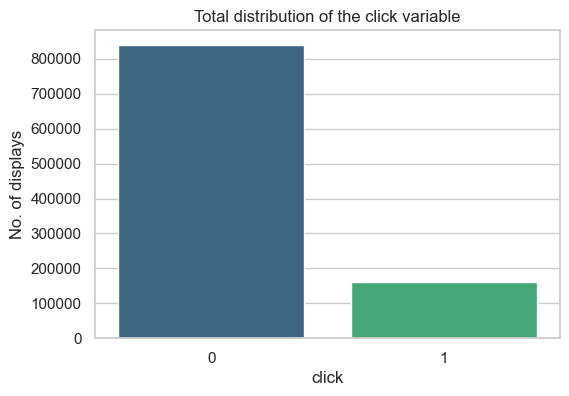
\includegraphics[width=0.7\linewidth]{figures/click_distribution.png}
\caption{\new{Avazu dataset:} Total distribution of the \texttt{click} variable.}
\label{fig:avazu_imbalance}
\end{figure}


\paragraph{High cardinality of categorical features}
\label{subsec:card}
The major challenge of the Avazu dataset is the high cardinality of its categorical features. Excluding the unique \texttt{id} column, the analysis showed that single features contain up to hundreds of thousands of unique values. As seen in Table~\ref{tab:cardinality}, within the $1,000,000$ rows sample, the \texttt{device\_ip} column contains $313,002$ unique values, \texttt{device\_id} contains $83,431$, and \texttt{device\_model} contains $4,581$ unique categories. Such dimensionality makes one-hot encoding computationally infeasible, which justifies the use of hashing techniques.  


\begin{table}[H]
\centering
\caption{\new{Avazu dataset:} Feature cardinality of the first 5 features.}
\label{tab:cardinality}
\begin{tabular}{|l|c|}
\hline
\textbf{Feature name} & \textbf{No. of unique values} \\
\hline
\texttt{id} & 1,000,000 \\
\texttt{device\_ip} & 313,002 \\
\texttt{device\_id} & 83,431 \\
\texttt{device\_model} & 4,581 \\
\texttt{app\_id} & 2,309 \\
\hline
\end{tabular}
\end{table}



\paragraph{CTR analysis}
Further analysis of the CTR has been conducted across different dimensions. The analysis made was as follows, as provided in Figure~\ref{fig:avazu_patterns}:

\begin{itemize}
    \item \textbf{Temporal variability (plot A):} The average CTR is not constant but fluctuates depending on the hour of the day. It suggests the presence of concept drift in the stream.
    \item \textbf{Device type influence (plot B):} The distribution of displays and clicks varies by \texttt{device\_type}. Even though one device dominates overall traffic, click rates vary by platform. 
    \item \textbf{Advertisement placement (plot C):} The analysis of the \texttt{banner\_pos} feature demonstrated a correlation between the physical placement of the banner on the screen and the resulting CTR.
\end{itemize}


\begin{figure}[H]
    \centering
    
    \begin{subfigure}{\linewidth}
        \centering
        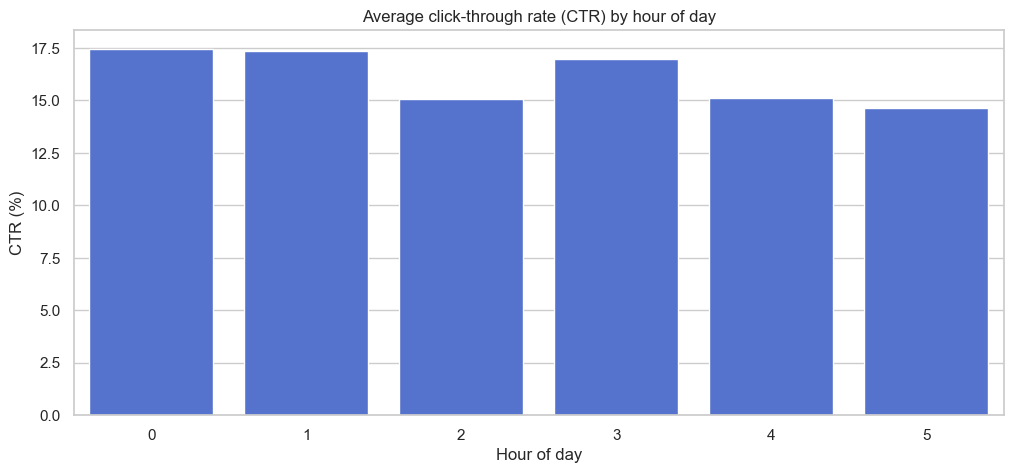
\includegraphics[width=0.75\linewidth]{figures/plot_a.png}
        \caption{\new{Avazu dataset:} Average CTR by hour of day}
        \label{fig:avazu_A}
    \end{subfigure}
    
    \vspace{0.5cm}
    
    \begin{subfigure}{0.48\linewidth}
        \centering
        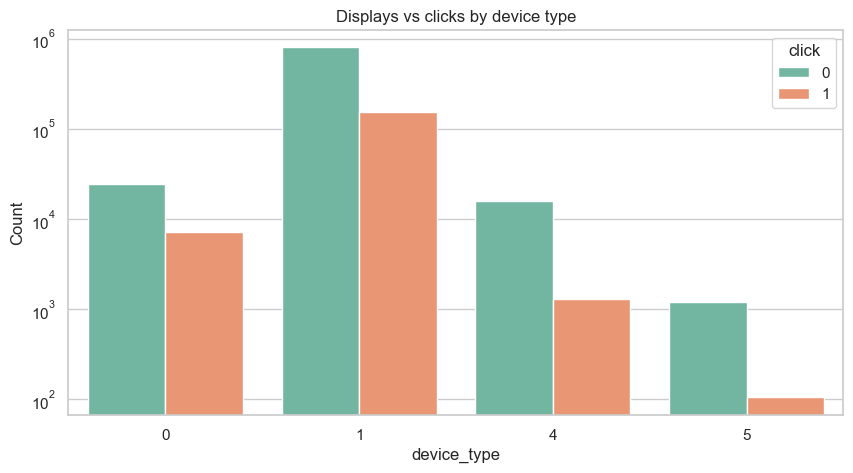
\includegraphics[width=\linewidth]{figures/plot_b.png}
        \caption{\new{Avazu dataset:} Displays vs clicks by device type}
        \label{fig:avazu_}
    \end{subfigure}
    \hfill
    \begin{subfigure}{0.48\linewidth}
        \centering
        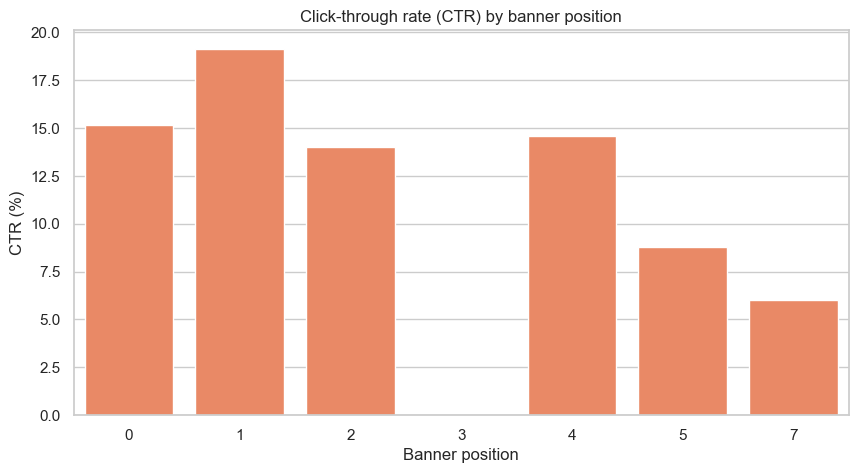
\includegraphics[width=\linewidth]{figures/plot_c.png}
        \caption{\new{Avazu dataset:} CTR by banner position}
        \label{fig:avazu_C}
    \end{subfigure}
    
    \caption{\new{Avazu dataset:} CTR analysis.}
    \label{fig:avazu_patterns}
\end{figure}


\subsubsection{Exploratory data analysis -- Criteo dataset}

The Criteo dataset is an online advertising dataset released by Criteo Labs\footnote{Criteo AI Lab, \textit{Criteo Research Datasets}, \url{https://ailab.criteo.com/ressources/}}. It contains feature values and click feedback for millions of display advertisements and serves as a widely used benchmark for CTR prediction. As in the Avazu dataset, we used the \texttt{train.txt} file, and $1,000,000$ records were analyzed. 

The dataset is heterogeneous and comprises 40 columns. The first attribute is the target variable (\texttt{label}), where 1 indicates the advertisement was clicked and 0 indicates it was not. The remaining 39 predictive attributes consist of 13 continuous numerical columns (\texttt{I1}--\texttt{I13}) and 26 anonymized categorical columns (\texttt{C1}--\texttt{C26}).


\paragraph{Target variable and class imbalance}
The target feature, \texttt{label}, is a binary variable representing user interactions. Once again, as presented in Figure~\ref{fig:criteo_imbalance}, the distribution analysis of the sampled records revealed a notable class imbalance. Particularly, 25.49\% of the impressions resulted in a click, while 74.51\% were ignored. Although the CTR is slightly higher compared to the Avazu dataset, the data remains heavily skewed ($P(Y=0) > P(Y=1)$) and we cannot use the traditional accuracy metrics.

\begin{figure}[H]
\centering
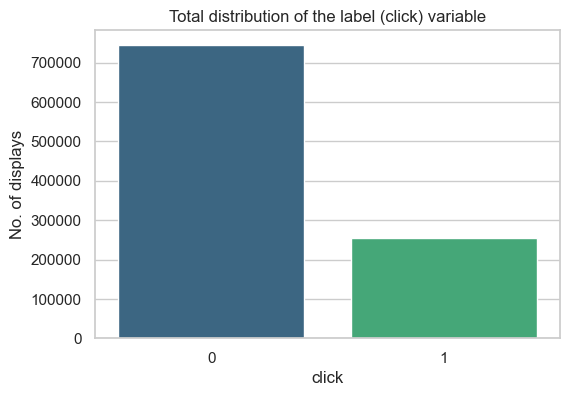
\includegraphics[width=0.7\linewidth]{figures/criteo_click_distrbution.png}
\caption{\new{Criteo dataset:} Total distribution of the \texttt{label} (click) variable.}
\label{fig:criteo_imbalance}
\end{figure}


\paragraph{Missing data and numerical skewness}
Unlike the Avazu dataset, the Criteo dataset poses the challenge of continuous variables. EDA showed that the numerical features (\texttt{I1}--\texttt{I13}) are sparsely populated, with varying percentages of missing values (NaNs) across columns. Furthermore, the existing continuous values exhibit highly right-skewed, long-tail distributions, as shown in Figure~\ref{fig:criteo_patterns}. They are populated by values close to zero but contain vivid outliers, as shown by truncating feature \texttt{I1} at the 99th percentile. The sparseness and skewness have required data preprocessing and an imputation strategy, such as filling missing numerical values with zeros, before model training.

\paragraph{High cardinality of categorical features}
The 26 categorical features (\texttt{C1}--\texttt{C26}) consist of 32-bit hashed strings. They exhibit a high cardinality similar to the Avazu dataset, despite the fact they have remained anonymized.

\begin{figure}[!htbp]
\centering
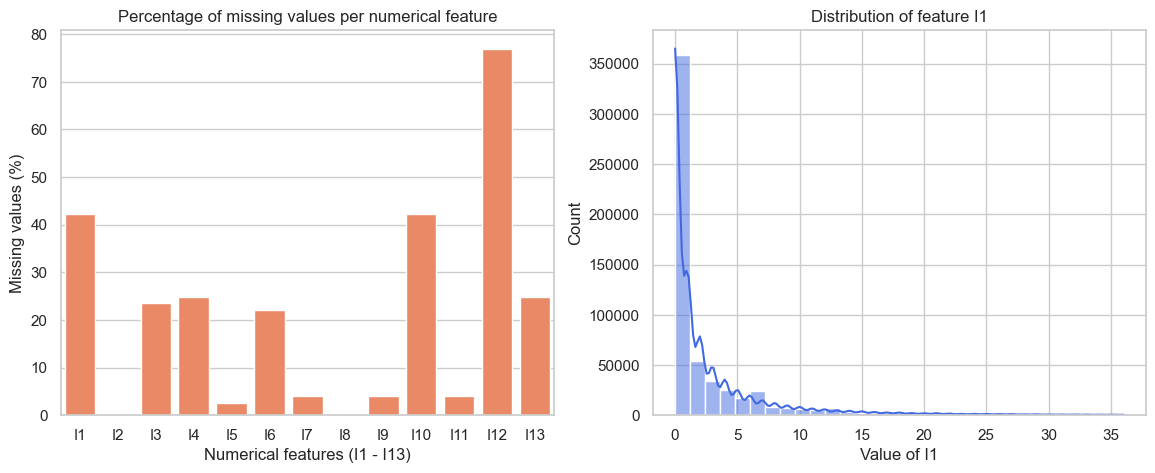
\includegraphics[width=\linewidth]{figures/missing_and_skew.png}
\caption{\new{Criteo dataset:} (A) Percentage of missing values per numerical feature, (B) Skewed distribution of continuous feature \texttt{I1}.}
\label{fig:criteo_patterns}
\end{figure}


\subsection{Feature engineering and hashing}
\label{subsec:feat}

As demonstrated in EDA, data streams with high cardinality and missing values can easily overload an online classifier's memory. To solve this, we have built a code that creates new features, reduces dimensionality, and saves the final output as an \texttt{ARFF} file for the Massive Online Analysis (MOA) framework \cite{bifet2010moa}.


\paragraph{Temporal and moving window features}
To help the model adapt to recent trends and concept drift, we have created dynamic features:
\begin{itemize}
    \item \textbf{Avazu:} \new{From the raw \texttt{hour} timestamp we derived five numeric time attributes: the hour of day, the day of month, the day of week, a binary weekend flag, and a coarse time-of-day bucket. We then created \emph{three} categorical interaction features, all following the same pattern \texttt{base}\,+\,\texttt{"\_h"}\,+\,hour-of-day, namely \texttt{site\_x\_hour}, \texttt{app\_x\_hour}, and \texttt{device\_x\_hour}. Their base columns \texttt{site\_id}, \texttt{app\_id}, and \texttt{device\_type} are raw (anonymised) Avazu categorical fields identifying, respectively, the publisher site, the application, and the device type on which the impression was shown; for example \texttt{site\_x\_hour}\,=\,\texttt{site\_id}\,+\,\texttt{"\_h"}\,+\,hour-of-day. These three interaction strings are appended to the list of categorical columns and passed to the feature hasher together with them, so each interaction is hashed as a single token rather than as a concatenation of already-hashed values; they are therefore absorbed into the 100 hashed columns and do not add extra numeric attributes. In addition, we added four numeric attributes derived from per-site and per-app rolling windows of length 1000: the recent site CTR and the recent app CTR (rolling click means grouped by \texttt{site\_id} and \texttt{app\_id}), the recent site frequency (rolling impression count per \texttt{site\_id}), and the site frequency change (the first difference of that rolling count). The three rolling statistics are shifted by one instance, and the frequency change is computed from the already-shifted count, so the current impression never contributes to its own feature value and no target leakage occurs.}
    \item \textbf{Criteo:} \new{The moving averages, standard deviations, and deviations from the mean were first computed on the raw numerical columns (\texttt{I1}--\texttt{I5}) using a sliding window of 1000 instances, with missing values skipped by the windowed estimator (\texttt{min\_periods=1}). Only after these statistics have been recorded, the remaining \texttt{NaN} values in the original columns have been replaced by zero. This order ensures that zero-imputed entries do not distort the window statistics.}
\end{itemize}


\paragraph{Dimensionality reduction via feature hashing}
As mentioned in Section~\ref{subsec:card}, techniques like one-hot encoding create too many columns for streaming data. Instead, we have decided to use the feature hashing algorithm \cite{weinberger2009feature} from \textit{scikit-learn} library to compress all categorical strings into a fixed-size vector of exactly 100 columns. This has provided two main benefits:
\begin{enumerate}
    \item The model's size stays the same, even if new, unseen categories appear in the stream.
    \item By keeping the number of columns strictly bounded, the SRP ensemble can process data much more quickly.
\end{enumerate}

\paragraph{Final state}
In the final step, we have merged all these parts together. For Avazu, we have combined \new{the five numeric time attributes and the four numeric sliding-window attributes (nine numeric features in total)} with the 100 hashed columns\new{, which gives the 109 Avazu features reported in Table~\ref{tab:datasets_summary}}. For Criteo on the other hand, we have combined the 13 original numeric columns, the 15 new moving statistics, and the 100 hashed columns. This optimized data has then been used to train and evaluate our models.


\subsection{\new{Synthetic data streams}}
\label{subsec:synth}

\new{Real-world streams contain natural, hidden concept drifts, but controlled synthetic streams are necessary to verify whether an adaptation mechanism reacts correctly when the drift location and drift type are known. In response to the reviewer comment, the final evaluation was extended from the original Agrawal-only synthetic setup to five synthetic stream configurations. Every synthetic run contains 200,000 instances and places the main drift at instance 100,000.}

\paragraph{\new{Agrawal variants}}
\new{The Agrawal generator \cite{agrawal1993database} simulates a loan-approval process using 9 predictive attributes. We use three variants: \texttt{agrawal\_sudden}, where the classification function switches abruptly from function 1 to function 3; \texttt{agrawal\_gradual}, where the same concept change is spread over a 40,000-instance transition window; and \texttt{agrawal\_noisy}, where a sudden function change is combined with 10\% perturbation noise. These variants test whether the models remain stable under abrupt, gradual, and noisy drift.}

\paragraph{\new{LED irrelevant-attribute stream}}
\new{The \texttt{led\_irrelevant} stream is based on MOA's LED generator with 7 relevant digit-segment attributes and 17 irrelevant attributes. Before the drift, 3 relevant attributes are swapped with irrelevant ones; after the drift, 7 attributes are swapped. This stream directly tests whether feature-selection mechanisms can cope with a changing set of relevant and irrelevant attributes. Since LED is a 10-class stream, the AUC values reported for this dataset should be interpreted cautiously; the main metrics used for comparison are Accuracy, Log Loss, and windowed Log Loss.}

\paragraph{\new{High-dimensional RBF stream}}
\new{The \texttt{rbf\_highdim} stream uses two MOA Random RBF concepts with 100 numeric attributes, 2 classes, and 50 centroids. The stream switches from seed 1 to seed 2 at the drift point. This satisfies the reviewer's request for a larger-dimensional synthetic stream and tests whether the proposed method behaves sensibly when the feature space is closer to the dimensionality of the real hashed CTR streams.}


\subsection{Summary of data streams characteristics}
\label{subsec:summ}

\new{Following the EDA, feature engineering, dimensionality reduction, and synthetic-stream extension phases, seven data streams were evaluated sequentially in the Java/MOA pipeline. Table~\ref{tab:datasets_summary} presents the final characteristics of the streams used in the 200,000-instance final evaluation.}

\begin{table}[!htbp]
\centering
\caption{\new{Summary of the final data streams used for model evaluation.}}
\label{tab:datasets_summary}
\resizebox{\linewidth}{!}{%
\begin{tabular}{|l|c|l|c|l|}
\hline
\textbf{Dataset} & \textbf{Instances per run} & \textbf{Final feature types} & \textbf{Feature count} & \textbf{Concept drift type} \\
\hline
\textbf{Avazu} & \new{200,000} & Numeric + hashed categorical & 109 & Natural CTR drift \\
\hline
\textbf{Criteo} & \new{200,000} & Continuous + hashed categorical & 128 & Natural CTR drift \\
\hline
\new{\textbf{Agrawal sudden}} & \new{200,000} & \new{Mixed synthetic} & \new{9} & \new{Abrupt function drift at 100,000} \\
\hline
\new{\textbf{Agrawal gradual}} & \new{200,000} & \new{Mixed synthetic} & \new{9} & \new{Gradual function drift centered at 100,000} \\
\hline
\new{\textbf{Agrawal noisy}} & \new{200,000} & \new{Mixed synthetic + noise} & \new{9} & \new{Abrupt function drift with 10\% perturbation noise} \\
\hline
\new{\textbf{LED irrelevant}} & \new{200,000} & \new{7 relevant + 17 irrelevant binary attributes} & \new{24} & \new{Relevant/irrelevant attribute swap at 100,000} \\
\hline
\new{\textbf{RBF highdim}} & \new{200,000} & \new{Numeric RBF features} & \new{100} & \new{Abrupt 100-dimensional concept switch at 100,000} \\
\hline
\end{tabular}%
}
\end{table}


\section{Evaluation methodology}
\subsection{Drift detection in real-time stream}
\label{subsec:drift}

First, we wanted to verify the presence of concept drift in the Avazu and Criteo datasets. To investigate it, we have used the ADWIN (ADaptive WINdowing) algorithm \cite{bifet2007learning, bifet2009adaptive}, implemented via the Python \texttt{river} library. It expands the window when the data are stationary and abruptly shrinks it when a statistically significant change in the stream's mean is detected.

\paragraph{Experiments}
We have processed the chronological sequences of both the Avazu and Criteo streams, using the ADWIN estimator to continuously monitor the moving average of the target variable. The CTR and the detected drift points are presented in Figure \ref{fig:adwin_avazu} and Figure \ref{fig:adwin_criteo}.

\begin{figure}[H]
\centering
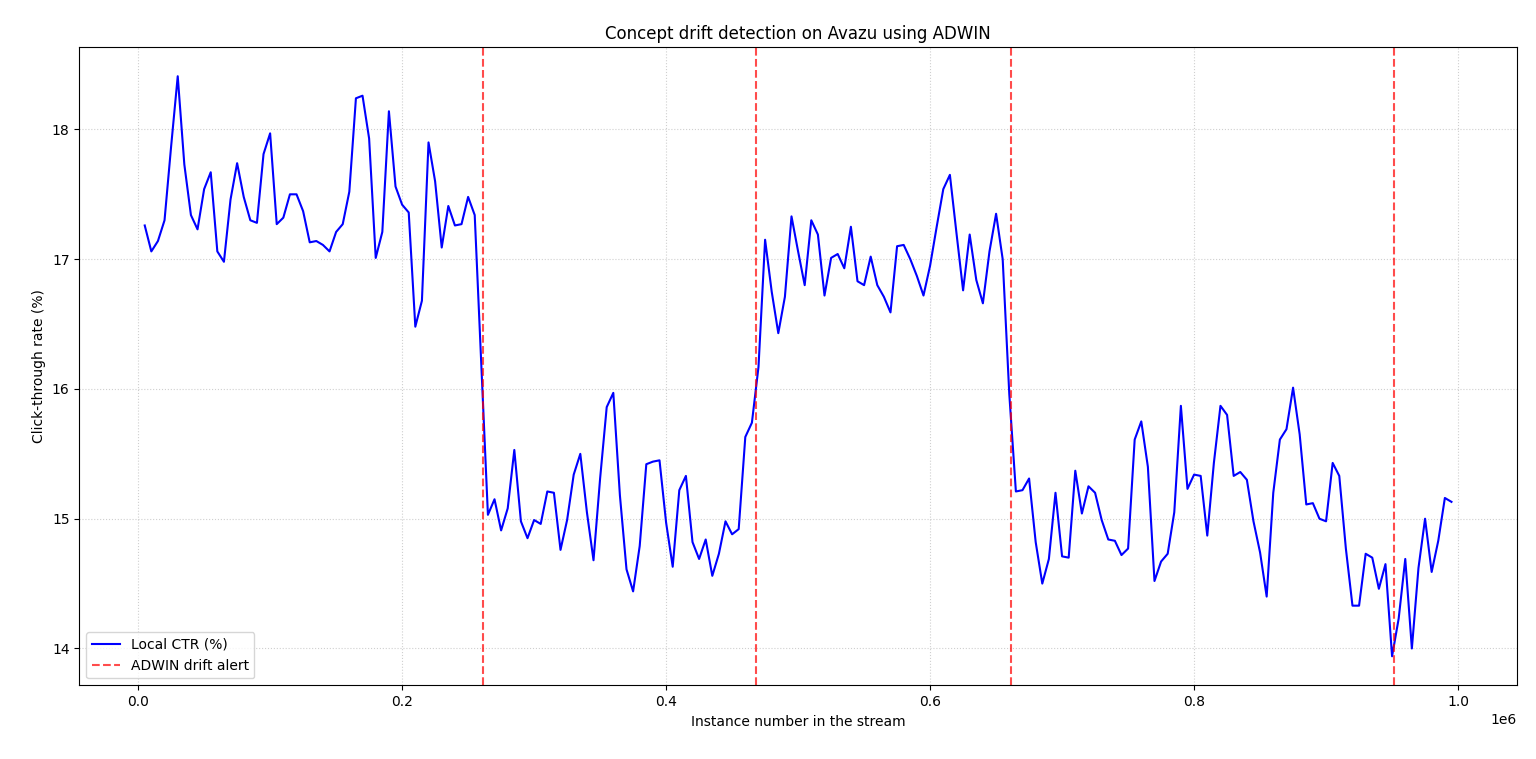
\includegraphics[width=\linewidth]{figures/CD_avazu.png}
\caption{\new{Avazu dataset:} Concept drift detection using the ADWIN algorithm.}
\label{fig:adwin_avazu}
\end{figure}

\begin{figure}[H]
\centering
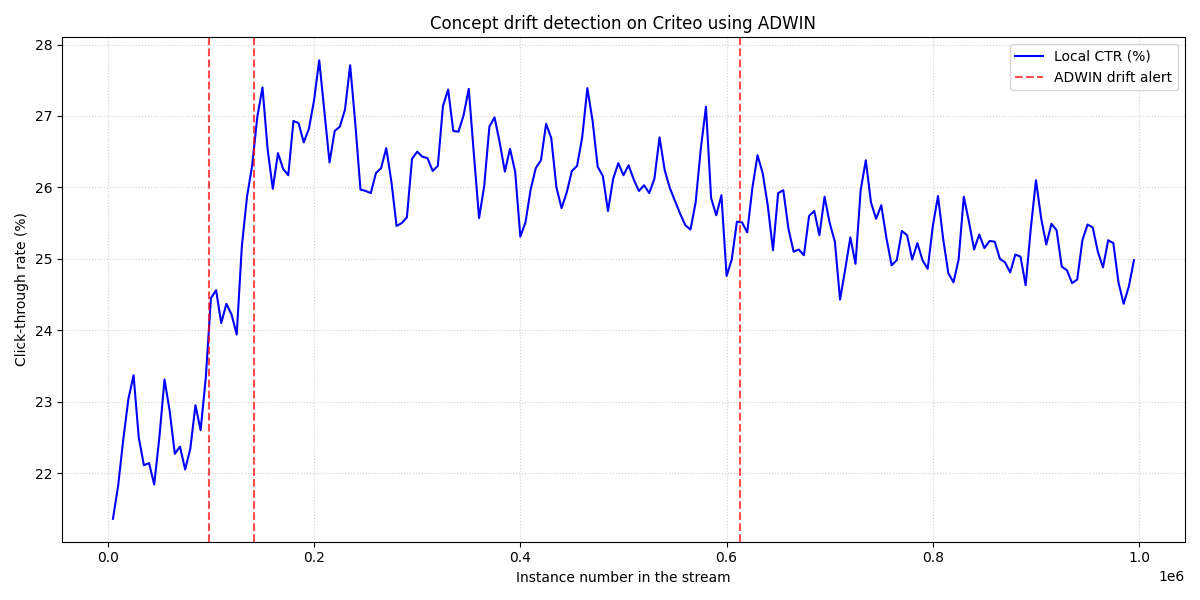
\includegraphics[width=\linewidth]{figures/CD_criteo.png}
\caption{\new{Criteo dataset:} Concept drift detection using the ADWIN algorithm.}
\label{fig:adwin_criteo}
\end{figure}

As shown in the above plots, the CTR is highly volatile and not constant over time. For the Avazu stream, the local CTR fluctuates between 14\% and 18.5\%, triggering four different drift alerts over $1,000,000$ points. Similarly, the Criteo stream shows non-stationarity. CTR climbs from initial values around 21\% up to almost 28\%, setting off three main drift alerts.

As we can see, the ADWIN detector has identified critical points in both datasets where the probability distribution underwent major shifts. Hence, the presence of concept drift in these streams requires us to use dynamic online learning models to maintain predictive performance. 

\new{It is crucial to note that monitoring the CTR (target variable) is not the only way to detect drift in these streams. Concept drift can also manifest itself as changes in the marginal distributions of individual input features (feature drift) or a deterioration in the prediction error rate of the trained model (error rate drift). Relying solely on the target variable can therefore allow us to miss drifts affecting feature importance without immediately changing the class ratio. Extended drift detection experiments based on model error rates and feature distributions are presented separately in the Section~\ref{sec:eval}.}

\subsection{Evaluation procedure in the MOA environment}
\label{subsec:eval_proc}

Due to the continuous nature of data streams, traditional machine learning evaluation techniques, such as cross-validation, are not applicable. We have used the prequential evaluation (test-then-train) method. In this approach, each incoming instance is first used to test the model -- generating a prediction -- and is then passed to the training algorithm to update the model's internal state. This means the classifier is always evaluated on unseen data. 

Both real-world streams show class imbalance. Hence, we have abandoned the standard accuracy metric, which favors the majority class. Instead, we decided to evaluate our models using logarithmic loss (Log Loss) and area under the ROC curve (AUC ROC) \cite{fawcett2006introduction}. The logarithmic loss heavily penalizes confident yet incorrect predictions, whereas the AUC-ROC evaluates the model's ability to correctly separate the positive (clicked) and negative (non-clicked) classes. 


\subsection{\new{Proof-of-concept baseline: HT in MOA}}
\label{subsec:poc}

\new{We first established a proof-of-concept baseline using the Hoeffding Tree (HT) -- a basic incremental decision tree for high-speed data streams. \new{The HT model was selected as the initial reference point because it is the simplest streaming tree learner: it grows splits incrementally but has no built-in drift-handling mechanism, which makes it a natural non-adaptive baseline against which adaptive methods can be compared.} The baseline HT model has been evaluated on our processed Avazu and Criteo streams using the prequential procedure. This preliminary evaluation was conducted in the MOA graphical interface and served to confirm that the data preprocessing produced sensible results before proceeding to the Java-based experiments described in Section~\ref{sec:archit} and Section~\ref{sec:eval}.}


\subsection{Adaptation gap on the synthetic stream}
\label{subsec:adapt}

We have evaluated a \new{HT} baseline on the synthetic Agrawal stream. \new{We have injected an abrupt concept drift (a switch from Agrawal classification function~1 to function~3) exactly at instance 100,000, consistent with the synthetic stream configuration used in the final evaluation.} Figure \ref{fig:adaptation_gap} illustrates the resulting adaptation gap.

\begin{figure}[H]
\centering

\includegraphics[width=\linewidth]{figures/adaptation_gap.png}
\caption{\new{Agrawal dataset:} Error of the baseline \new{HT} model over time, showing the adaptation gap after an abrupt concept drift. \new{Sudden drift takes place at instance 100,000.}}
\label{fig:adaptation_gap}
\end{figure}

\new{During the initial stable phase, from 0 to 100,000 instances, the HT has successfully learned the defined rules and has driven its classification error down to roughly 6\%. However, immediately upon drift injection, the previously learned tree splits became obsolete, causing the classification error to rise to a peak of about 10\%. Because a plain Hoeffding Tree cannot discard outdated splits, it can only recover by gradually growing new structure on top of the stale one, so the error decreases slowly back towards 8\% by the end of the stream.}

\new{The resulting rise-and-recovery forms a distinct triangular shape on the plot, whose width represents the recovery time ($t_{recovery}$).} This leaves us with an important observation. Namely, standard \new{non-adaptive} tree learning recovers from drift relatively slowly. Therefore, flattening this exact error curve and minimizing $t_{recovery}$ are our primary motives for investigating the dynamic OFS as the next milestone.


\section{Architecture of the proposed solution}
\label{sec:archit}

\subsection{Overall streaming pipeline}
\label{subsec:stream_pip}

The implementation in the repository follows the standard streaming-learning
loop: each instance is read in chronological order, transformed into a fixed
feature representation, predicted by the current model, scored, and only then
used for training. This protocol — known as prequential or test-then-train
evaluation \cite{gama2014survey} — prevents information leakage from future
observations into the current prediction and provides an unbiased estimate of
the model's behaviour as a function of stream position.

\begin{figure}[H]
\centering
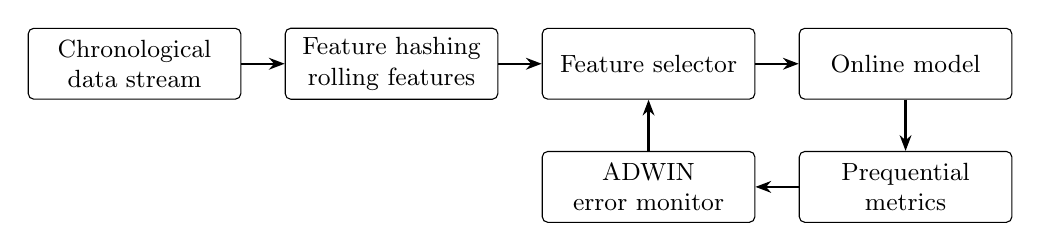
\begin{tikzpicture}[
    node distance=0.65cm and 0.55cm,
    every node/.style={font=\small},
    box/.style={draw, rounded corners=2pt, align=center, minimum width=2.7cm, minimum height=0.9cm},
    arrow/.style={-{Stealth[length=2mm]}, thick}
]
    \node[box] (stream) {Chronological\\data stream};
    \node[box, right=of stream] (features) {Feature hashing\\rolling features};
    \node[box, right=of features] (selector) {Feature selector};
    \node[box, right=of selector] (model) {Online model};
    \node[box, below=of model] (metrics) {Prequential\\metrics};
    \node[box, below=of selector] (adwin) {ADWIN\\error monitor};

    \draw[arrow] (stream) -- (features);
    \draw[arrow] (features) -- (selector);
    \draw[arrow] (selector) -- (model);
    \draw[arrow] (model) -- (metrics);
    \draw[arrow] (metrics) -- (adwin);
    \draw[arrow] (adwin) -- (selector);
\end{tikzpicture}
\caption{Architecture of the streaming evaluation and adaptation pipeline.}
\label{fig:system_architecture}
\end{figure}

The Java implementation is organised around five groups of classes. Stream
providers load either ARFF-based real datasets or the \new{Agrawal, LED, and
Random RBF synthetic streams} through a unified \texttt{StreamProvider}
interface. Model wrappers expose a
common \texttt{StreamModel} contract for Hoeffding Tree, Hoeffding Adaptive
Tree, SRP, and the proposed drift-aware SRP model. Feature selectors implement
no selection, static top-K selection, periodic online ranking, and the
drift-aware selection introduced in this work. The prequential evaluator
coordinates prediction, metric updates, drift detection, model training, and
CSV logging in a single integration loop. Decoupling the components through
interfaces makes it possible to evaluate any combination of provider, selector
and model without modifying the evaluator itself.

\begin{algorithm}[H]
\color{blue}
\caption{\new{Main prequential evaluation and adaptation pipeline}}
\KwIn{Chronological stream $S$, feature selector $F$, stream model $M$, drift detector $D$, metrics $\mathcal{M}$}
\KwOut{Metric history, final metrics, detected drift events}
Initialise $F$ on the stream header\;
Initialise $M$ on the filtered header returned by $F$\;
Reset all metrics and reset $D$\;
\ForEach{incoming instance $(x_t,y_t)$ in chronological order}{
    $\tilde{x}_t \leftarrow F.\mathrm{filter}(x_t)$\;
    $\hat{p}_t \leftarrow M.\mathrm{predictProbability}(\tilde{x}_t)$\;
    Update every metric in $\mathcal{M}$ using $(\hat{p}_t,y_t)$\;
    $e_t \leftarrow \mathbb{1}[\mathbb{1}(\hat{p}_t \geq 0.5) \neq y_t]$\;
    \If{$D.\mathrm{detect}(e_t)$}{
        Store a drift event at time $t$\;
        Signal the drift to the feature selector $F$ (freeze its pre-drift statistics)\;
    }
    Train $M$ on $(\tilde{x}_t,y_t)$\;
    Update the feature selector buffer with the raw instance $(x_t,y_t)$\;
    \If{$F$ emits a new feature subset (its post-drift window is complete)}{
        Rebuild the filtered header from the new subset\;
        \eIf{$M$ is a monolithic model (HT, HAT, or vanilla SRP)}{
            Reinitialise $M$ on the new filtered header, dropping the obsolete splits\;
        }{
            Repair only the affected DASRP subspaces and reinitialise those learners\;
        }
    }
    \If{$t$ is a logging point}{
        Store the current metric snapshot\;
    }
}
\label{alg:main_pipeline}
\end{algorithm}

\subsection{Baseline models and feature selectors}
\label{subsec:baseline}

The baseline model set contains Hoeffding Tree (HT), Hoeffding Adaptive Tree
(HAT), and Streaming Random Patches (SRP). HT is the basic incremental tree
model for high-speed streams \cite{hulten2001mining} and serves as a
non-adaptive reference. HAT extends the tree with ADWIN-based monitors at
internal nodes and replaces obsolete subtrees with alternative subtrees as the
underlying concept changes. SRP is an ensemble method designed for evolving
streams \cite{gomes2019streaming}; it combines online bagging with random
feature subspaces and per-learner drift detection. In the repository, the SRP
baseline uses 10 trees and a 60\% random subspace setting, consistent with the
default values used by the original authors.

Three baseline feature-selection strategies were implemented and evaluated.
\new{In all selectors, Information Gain is computed on the selector's current
sample buffer, not on the full future stream. Static top-K uses the initial
5,000-instance warm-up buffer; online ranking uses the most recent
5,000-instance sliding buffer; drift-aware selection uses one pre-drift and one
post-drift buffer. For each feature $X_i$, the ranker computes
$IG(X_i;Y)=H(Y)-H(Y\mid X_i)$ with respect to the observed class attribute
$Y$. Nominal attributes use empirical class counts per value, while numeric
attributes are discretised into 10 data-dependent bins before conditional
entropy is estimated.}

\begin{itemize}
    \item \textbf{No selector}: all attributes are passed to the model. This
    is the natural reference for measuring whether feature selection helps at
    all on a given stream.
    \item \textbf{Static top-K}: Information Gain is estimated on a warm-up
    segment of 5,000 instances and the selected features remain fixed for the
    rest of the stream.
    \item \textbf{Online ranking}: Information Gain is recomputed on a sliding
    window of 5,000 instances every 5,000 instances. The selected feature set
    therefore evolves with the stream, but only on a fixed schedule.
\end{itemize}

These baselines isolate the contribution of dynamic feature selection from
the contribution of the classifier itself, and provide a comparison point for
the proposed drift-aware variants.

\new{Feature selection influences all non-DASRP models through the instance
header passed to the classifier. The selector physically filters the incoming
instance to the currently selected attributes and appends the class attribute at
the end. Therefore HT, HAT, and vanilla SRP never receive attributes outside
the selected subset. When a dynamic selector changes the subset, the affected
monolithic model is reinitialised on the new filtered header. Past tree splits
are not retroactively constrained to the newly selected features; instead, the
old model state is dropped and a new model starts learning from the new feature
space. Static top-K does not trigger later resets because its selected subset is
fixed after warm-up.}

\subsection{Drift-aware feature selection}
\label{subsec:drift-aware}

The proposed drift-aware selector replaces the periodic schedule of the online
ranking baseline with an event-driven adaptation triggered by ADWIN. The key
observation is that the meaningful signal for feature selection is not the
absolute Information Gain at a single point in time, but rather the change in
Information Gain caused by the drift itself: features whose predictive value
has dropped should be replaced precisely by features whose predictive value
has risen.

The selector maintains a sliding buffer of recent instances. While no drift
is signalled, the buffer simply rolls forward. When ADWIN raises a drift
alert, the selector freezes the current buffer as the pre-drift snapshot and
records the corresponding Information Gain values $IG_{before}$. It then
continues to consume instances normally for one further window, accumulating
post-drift data. Once the post-drift window is full, $IG_{after}$ is computed
and the per-feature change is taken as
\[
\Delta IG_i \;=\; IG_{after,i} - IG_{before,i}.
\]
Features for which $\Delta IG_i$ exceeds a positive threshold are treated as
strengthened; features for which it falls below the symmetric negative
threshold are treated as weakened. The new selected set is obtained from the
current top-$K$ ranking by adding strengthened candidates and removing
weakened ones, with a length correction that brings the result back to size
$K$ if either operation overshoots.

\new{For Avazu, Criteo, and the high-dimensional RBF stream, the selector
keeps 20 features. For the Agrawal variants, where the feature space is small,
it keeps 5 features. For the LED stream, it keeps 7 features. This value
coincides with the number of relevant LED-segment attributes; because that count
is part of the synthetic generator's ground truth and would be unknown on a real
stream, we treat it as an oracle-informed setting and read the LED run as a
controlled diagnostic of feature-relevance handling rather than as a label-free
benchmark (see Section~\ref{subsec:drift_aware_srp}). Real CTR and RBF experiments
use a 5,000-instance comparison window; Agrawal uses an 800-instance window;
LED uses a 1,000-instance window. These values reflect the different
dimensionality and drift dynamics of the streams.}

\new{The ADWIN input in this part of the pipeline is a single scalar error
stream per evaluated model, not one ADWIN detector per feature. After each
prediction, the evaluator sends $e_t=0$ for a correct binary decision and
$e_t=1$ for an incorrect one. The ADWIN alarm therefore means that the model's
recent error rate changed significantly. Feature-level changes are inferred
after the alarm by comparing $IG_{before}$ and $IG_{after}$ on buffered
instances.}

\begin{algorithm}[H]
\color{blue}
\caption{\new{Drift-aware feature selection after an ADWIN alarm}}
\KwIn{Recent buffer $B$, currently selected set $S_{old}$, top-$K$ size $K$, post-drift window length $W$, threshold $\tau$}
\KwOut{Updated selected set $S_{new}$, removed features $R$, added features $A$}
\If{ADWIN raises an alarm and no adaptation is already pending}{
    Freeze the current buffer as $B_{before}$\;
    Compute $IG_{before}(i)$ for every feature $i$ on $B_{before}$\;
    Clear the rolling buffer and start collecting post-drift data\;
}
\If{$W$ post-drift instances have been collected}{
    Let $B_{after}$ be the collected post-drift buffer\;
    Compute $IG_{after}(i)$ for every feature $i$ on $B_{after}$\;
    Compute $\Delta IG_i = IG_{after}(i)-IG_{before}(i)$\;
    $S_{base}\leftarrow$ top-$K$ features ranked by $IG_{after}$\;
    $S_{new}\leftarrow S_{base}$\;
    Add to $S_{new}$ every feature with $\Delta IG_i>\tau$\;
    Remove from $S_{new}$ every feature with $\Delta IG_i<-\tau$\;
    \lIf{$|S_{new}|>K$}{keep in $S_{new}$ the $K$ features with the highest $IG_{after}$}
    \lIf{$S_{new}=\emptyset$}{$S_{new}\leftarrow S_{base}$}
    Compute $R\leftarrow S_{old}\setminus S_{new}$ and $A\leftarrow S_{new}\setminus S_{old}$\;
    $S_{old}\leftarrow S_{new}$\;
    Rebuild the filtered header from $S_{new}$ and notify the model adaptation listener\;
}
\label{alg:drift_aware_selector}
\end{algorithm}

\new{This update rule also prevents a feature with low absolute Information
Gain from replacing a feature that remains highly informative merely because
the low-IG feature is improving. The candidate set is anchored in the
post-drift top-$K$ ranking and, whenever the set grows beyond $K$, it is
shrunk again according to $IG_{after}$. Therefore a low but growing feature can
enter only when it has become competitive after the drift or when another
selected feature has genuinely weakened.}

\new{Figure~\ref{fig:drift_aware_selector_flow} summarises the control flow of
the drift-aware selector as an event-driven, two-phase process.}

\begin{figure}[H]
\centering
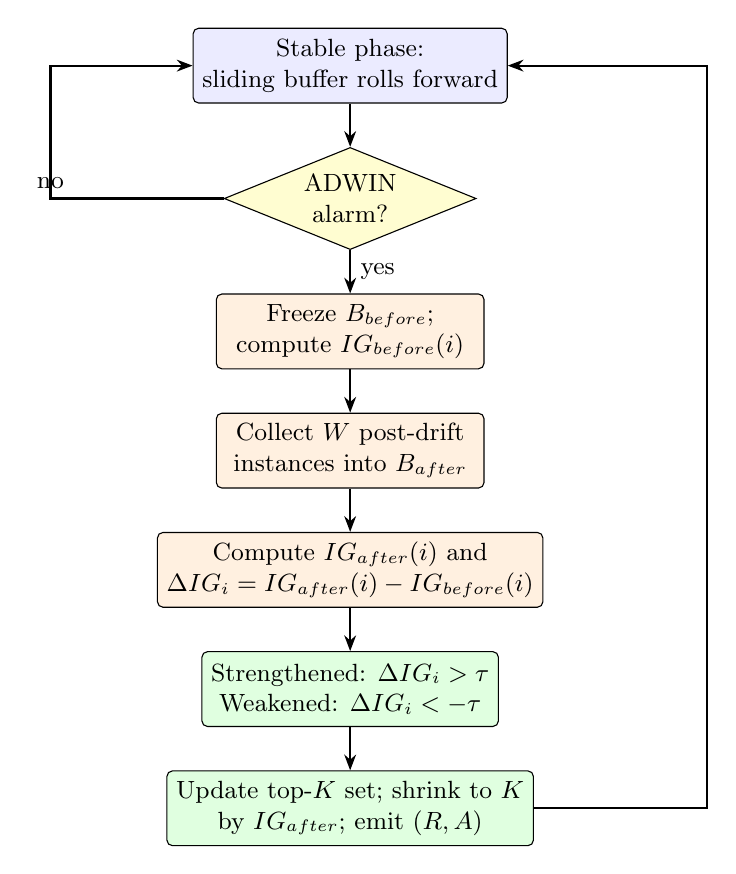
\begin{tikzpicture}[
    node distance=0.55cm and 0.9cm,
    every node/.style={font=\small},
    box/.style={draw, rounded corners=2pt, align=center,
                minimum width=3.4cm, minimum height=0.95cm},
    stable/.style={box, fill=blue!8},
    freeze/.style={box, fill=orange!12},
    act/.style={box, fill=green!12},
    dec/.style={draw, diamond, aspect=2, align=center, fill=yellow!18,
                inner sep=1pt, minimum width=3.2cm},
    arrow/.style={-{Stealth[length=2mm]}, thick}
]
    \node[stable] (roll) {Stable phase:\\sliding buffer rolls forward};
    \node[dec, below=of roll] (alarm) {ADWIN\\alarm?};
    \node[freeze, below=of alarm] (before)
        {Freeze $B_{before}$;\\compute $IG_{before}(i)$};
    \node[freeze, below=of before] (collect)
        {Collect $W$ post-drift\\instances into $B_{after}$};
    \node[freeze, below=of collect] (after)
        {Compute $IG_{after}(i)$ and\\$\Delta IG_i = IG_{after}(i) - IG_{before}(i)$};
    \node[act, below=of after] (split)
        {Strengthened: $\Delta IG_i > \tau$\\Weakened: $\Delta IG_i < -\tau$};
    \node[act, below=of split] (rebuild)
        {Update top-$K$ set; shrink to $K$\\by $IG_{after}$; emit $(R, A)$};

    \draw[arrow] (roll) -- (alarm);
    \draw[arrow] (alarm) -- node[right]{yes} (before);
    \draw[arrow] (alarm.west) -- ++(-2.2,0) node[above]{no} |- (roll.west);
    \draw[arrow] (before) -- (collect);
    \draw[arrow] (collect) -- (after);
    \draw[arrow] (after) -- (split);
    \draw[arrow] (split) -- (rebuild);
    \draw[arrow] (rebuild.east) -- ++(2.2,0) |- (roll.east);
\end{tikzpicture}
\caption{\new{Control flow of the drift-aware feature selector
(Algorithm~\ref{alg:drift_aware_selector}). While stable, the buffer simply
rolls forward; an ADWIN alarm freezes the pre-drift Information Gain, a further
window of $W$ instances is collected, and the selected set is updated from the
signed Information Gain change $\Delta IG_i$.}}
\label{fig:drift_aware_selector_flow}
\end{figure}

\subsection{Drift-Aware SRP}
\label{subsec:drift_aware_srp}

The proposed model, Drift-Aware SRP (DASRP), extends the SRP framework along
two complementary axes. First, ensemble subspaces become responsive to
feature drift instead of being fixed at construction time. Second, \new{members
whose subspaces are most heavily affected by the drift do not vote at full
strength immediately:} the ensemble keeps track of how much fresh evidence each
\new{such} member has seen and weighs its vote accordingly during recovery.
Both mechanisms are designed to
avoid the failure mode of a naive reset, in which the ensemble loses all
accumulated knowledge on every drift event.

The implementation is split between two helper classes used by DASRP. The
\texttthyphen{SubspaceManager} owns the per-learner feature subsets and exposes an
\texttt{adaptSubspaces} operation that consumes the weakened and strengthened
feature sets produced by the drift-aware selector. For each learner, it
counts the number of weakened features inside its subspace; learners below a
configurable overlap threshold are left untouched, since their predictive
basis was not affected by the drift. Learners above the threshold have their
weak features replaced, preferring strengthened candidates and falling back
to neutral features when the strengthened pool is too small. \new{Every learner
whose subspace is actually modified is then reinitialised on its new
sub-header, since a Hoeffding tree built on the old attribute set cannot be
reused consistently once that attribute set changes. The reset ratio does
\emph{not} decide whether a learner is reinitialised; instead, the fraction of
the original subspace that had to be replaced is compared against the reset
ratio only to decide which of the reinitialised learners are additionally
flagged for voting-weight reduction during recovery.}

\new{Formally, let $S_m$ be the current subspace of learner $m$ and $W$ the
weakened feature set emitted by the selector. The learner is adapted only if it
shares at least $\omega$ weak features,
\[
|S_m \cap W| \;\geq\; \omega \quad (\text{minimum overlap}),
\]
and, once adapted, it is additionally flagged for weight reduction when the
weakened fraction of its old subspace reaches the reset ratio $\rho$,
\[
o_m \;=\; \frac{|S_m \cap W|}{|S_m|} \;\geq\; \rho .
\]
In our experiments $\omega \in \{1,2\}$ and $\rho = 0.5$.}

The \texttt{WeightManager} mirrors \new{this weight} decision on the voting side.
Members \new{flagged by the subspace manager as exceeding the reset ratio} have their weight reduced
to a configurable value (0.3 in our experiments) and recover linearly toward
the normal weight 1.0 at a fixed rate per training instance. Aggregation is
performed as a weighted average,
\[
\hat{p} \;=\; \frac{\sum_{i=1}^{N} w_i \, p_i}{\sum_{i=1}^{N} w_i},
\]
so that freshly reset members influence the ensemble in proportion to the
amount of new data they have processed. \new{A flagged learner $m$ has its
weight set to $w_{\text{reset}}$ at the reset instant $t_m^{0}$ and then recovers
linearly,
\[
w_m(t) \;=\; \min\!\bigl(w_{\text{norm}},\; w_{\text{reset}} + r\,(t - t_m^{0})\bigr),
\]
with $w_{\text{reset}} = 0.3$, $w_{\text{norm}} = 1.0$, and recovery rate
$r = 0.001$ per instance.} With a recovery rate of 0.001 per
instance, full recovery takes roughly $\tfrac{w_{\text{norm}} - w_{\text{reset}}}{r} = 700$ instances, which is comparable to
the data volume needed by a Hoeffding tree to perform its first split.

\new{DASRP can remove a feature from a learner only when that feature appears
in the selector's weakened set and the learner contains enough weakened
features to pass the overlap threshold. Thus, potentially relevant features are
not globally removed from the whole ensemble at once: unaffected learners keep
their old subspaces and continue voting. The final experiments show that this
selective repair is useful on high-dimensional CTR streams, but simple
synthetic streams with frequent ADWIN alarms can still cause over-adaptation.
For this reason, stricter thresholds and per-stream calibration are treated as
part of the final recommendations rather than as a universal default.}

The adaptation cycle ties everything together as follows:

\begin{enumerate}
    \item ADWIN detects a change in the online error stream.
    \item The drift-aware selector compares Information Gain before and after
    the drift and emits the weakened and strengthened feature sets.
    \item The \texttt{SubspaceManager} removes weak features from affected
    subspaces and fills the gaps using strengthened features whenever possible.
    \item \new{Every learner whose subspace was modified is reinitialised on
    its new sub-header.}
    \item \new{Learners whose replaced fraction exceeds the reset ratio are
    additionally} flagged \new{for weight reduction; the \texttt{WeightManager}
    lowers their vote weight} and gradually restores it during the subsequent
    training instances.
\end{enumerate}

\new{Figure~\ref{fig:dasrp_flow} shows how a single ADWIN alarm is turned into a
per-learner repair-or-keep decision and the subsequent weighted vote.}

\begin{figure}[H]
\centering
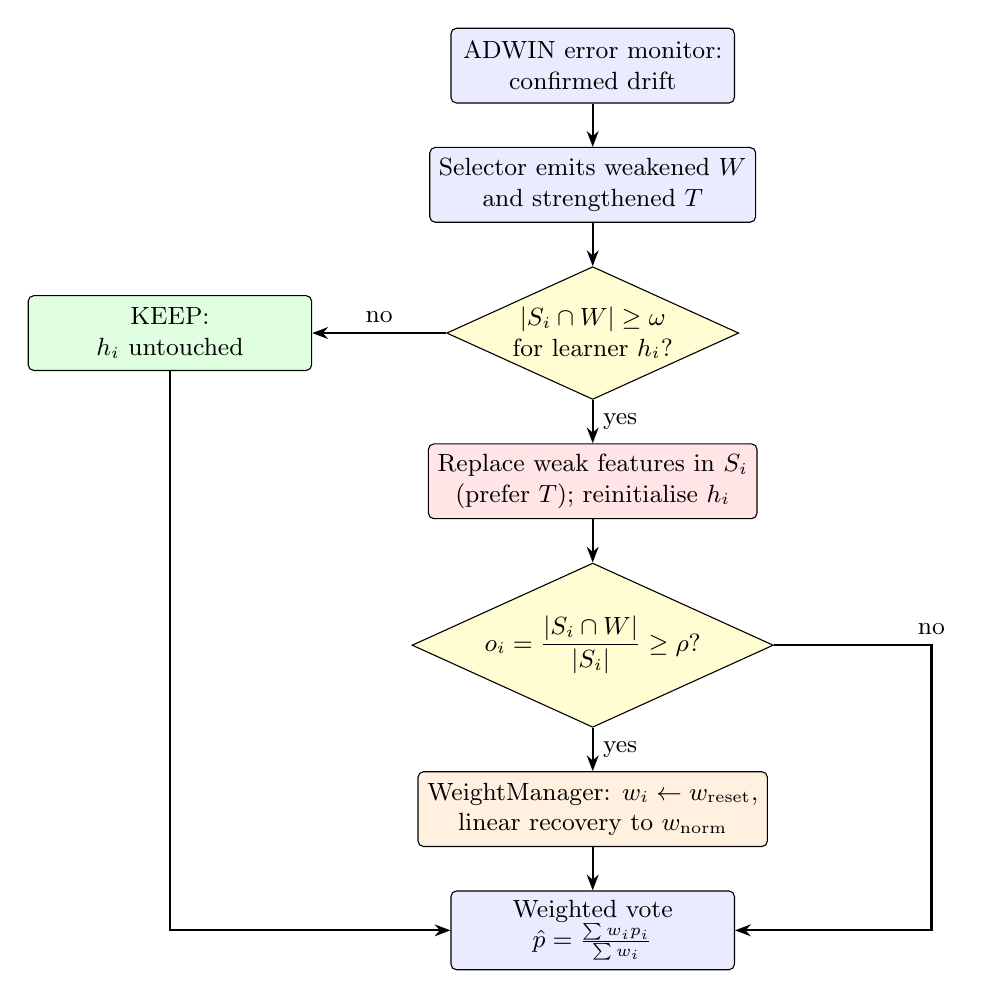
\begin{tikzpicture}[
    node distance=0.55cm and 0.7cm,
    every node/.style={font=\small},
    box/.style={draw, rounded corners=2pt, align=center,
                minimum width=3.6cm, minimum height=0.95cm},
    src/.style={box, fill=blue!8},
    dec/.style={draw, diamond, aspect=2.2, align=center, fill=yellow!18,
                inner sep=1pt, minimum width=3.4cm},
    keep/.style={box, fill=green!12},
    rep/.style={box, fill=red!10},
    wm/.style={box, fill=orange!12},
    arrow/.style={-{Stealth[length=2mm]}, thick}
]
    \node[src] (adwin) {ADWIN error monitor:\\confirmed drift};
    \node[src, below=of adwin] (sel)
        {Selector emits weakened $W$\\and strengthened $T$};
    \node[dec, below=of sel] (test)
        {$|S_i \cap W| \geq \omega$\\for learner $h_i$?};
    \node[keep, left=1.7cm of test] (keep)
        {KEEP:\\$h_i$ untouched};
    \node[rep, below=of test] (repair)
        {Replace weak features in $S_i$\\ (prefer $T$); reinitialise $h_i$};
    \node[dec, below=of repair] (reset)
        {$o_i = \dfrac{|S_i \cap W|}{|S_i|} \geq \rho$?};
    \node[wm, below=of reset] (weight)
        {WeightManager: $w_i \leftarrow w_{\text{reset}}$,\\linear recovery to $w_{\text{norm}}$};
    \node[box, fill=blue!8, below=of weight] (vote)
        {Weighted vote\\$\hat{p} = \frac{\sum w_i p_i}{\sum w_i}$};

    \draw[arrow] (adwin) -- (sel);
    \draw[arrow] (sel) -- (test);
    \draw[arrow] (test) -- node[above]{no} (keep);
    \draw[arrow] (test) -- node[right]{yes} (repair);
    \draw[arrow] (repair) -- (reset);
    \draw[arrow] (reset) -- node[right]{yes} (weight);
    \draw[arrow] (reset.east) -- ++(2.0,0) node[above]{no} |- (vote.east);
    \draw[arrow] (weight) -- (vote);
    \draw[arrow] (keep.south) |- (vote.west);
\end{tikzpicture}
\caption{\new{DASRP adaptation cycle. After a confirmed drift, each learner
$h_i$ is kept untouched when its subspace overlaps the weakened set by fewer
than $\omega$ features; otherwise its weak features are replaced and the learner
is reinitialised. Only learners whose weakened fraction $o_i$ reaches the reset
ratio $\rho$ have their voting weight reduced and then linearly recovered. The
ensemble prediction is the weight-normalised average of the member
probabilities.}}
\label{fig:dasrp_flow}
\end{figure}

DASRP uses online bagging with $\lambda=1$ rather than
the $\lambda=6$ value of the reference SRP implementation; this reduces the
amplification of repeated training and keeps the focus of the experiments on
the contribution of the drift-aware components. Drift detection is handled at
the ensemble level by the external ADWIN monitor rather than by per-learner
detectors, which keeps the adaptation policy concentrated in a single place.

\new{On real CTR datasets, DASRP uses 10 base Hoeffding-tree learners,
subspaces of size 20, ADWIN with $\delta=0.002$, reset weight 0.3, recovery
rate 0.001, and a reset ratio of 0.5. On Agrawal variants, the configuration
uses subspaces of size 4, ADWIN with $\delta=0.001$, reset weight 0.5, and
recovery rate 0.005. On LED, the subspace size is 7. We note that this equals
the number of relevant LED-segment attributes; since that number is known only
because LED is a synthetic generator, choosing the subspace size from it is an
oracle-informed setting that would not be available on a real stream. We
therefore report the LED result as a controlled diagnostic of how the method
handles irrelevant attributes, not as a label-free comparison, and flag this as
a limitation. On the high-dimensional
RBF stream, the subspace size is 20, matching the real CTR setting. The
different settings reflect the feature-space size and drift dynamics of each
stream family.}

\section{Final evaluation}
\label{sec:eval}

\subsection{Experiment matrix}
\label{subsec:matrix}

The final evaluation used the CSV outputs from the implemented Java experiment
pipeline. \new{The baseline matrix contains 63 runs: 7 datasets, 3 models
(HT, HAT, SRP), and 3 feature selectors (none, static top-K, online ranking).
The drift-aware matrix contains 21 additional runs: for each dataset, HT with
the drift-aware selector, HAT with the drift-aware selector, and DASRP. In
total, the report summarizes 84 prequential experiments. The seven datasets are
Avazu, Criteo, Agrawal sudden, Agrawal gradual, Agrawal noisy, LED
irrelevant-attribute drift, and high-dimensional RBF.}

Each run processes 200,000 instances. Metrics are logged every 1,000 instances.
The main metrics are final Accuracy, final Log Loss, final AUC, and windowed
1,000-instance Log Loss. Log Loss is the most important metric for CTR
prediction because the output probability is used directly in ranking and
bidding decisions.
\new{AUC is treated as a secondary metric. It is directly comparable for the
binary CTR, Agrawal, and RBF streams. For the 10-class LED stream, the
implementation effectively reports a class-1-versus-rest AUC, so LED results
are interpreted primarily through Accuracy, Log Loss, and windowed Log Loss.}

\subsection{Real CTR results}
\label{subsec:ctr_res}

\begin{table}[H]
\centering
\caption{Final metrics on real CTR streams (\new{Avazu, Criteo}). \new{The lower Log Loss, the better.}}
\label{tab:real_final_metrics}
\begin{tabular}{llccc}
\toprule
Dataset & Method & Accuracy & Log Loss & AUC \\
\midrule
Avazu & \new{HT + no selector} & \new{0.8052} & \new{1.0169} & \new{0.6339} \\
Avazu & \new{SRP + online ranking} & \new{0.8206} & \new{0.4889} & \new{0.6615} \\
Avazu & SRP + static top-K & 0.8243 & 0.4659 & 0.7022 \\
Avazu & \textbf{DASRP + drift-aware SRP} & \textbf{0.8253} & \textbf{0.4332} & \textbf{0.7048} \\
\midrule
Criteo & \new{HT + no selector} & \new{0.7497} & \new{1.0110} & \new{0.6297} \\
Criteo & \new{SRP + online ranking} & \new{0.7561} & \new{0.5513} & \new{0.6585} \\
Criteo & \textbf{DASRP + drift-aware SRP} & \new{0.7579} & \new{\textbf{0.5294}} & \new{0.6669} \\
Criteo & \new{SRP + static top-K} & \new{\textbf{0.7654}} & \new{0.5562} & \new{\textbf{0.6865}} \\
\bottomrule
\end{tabular}
\end{table}

The most important result is that DASRP achieved the lowest final Log Loss on
both real CTR datasets. On Avazu, DASRP improved Log Loss from 0.4659 for the
best SRP baseline to 0.4332, which is a relative reduction of about 7.0\%. On
Criteo, \new{DASRP improved Log Loss from 0.5513 for the best SRP baseline
(online ranking) to 0.5294, a relative reduction of about 4.0\%}. This supports the hypothesis that drift-aware feature adaptation is
useful in high-dimensional CTR streams.

\begin{figure}[H]
\centering
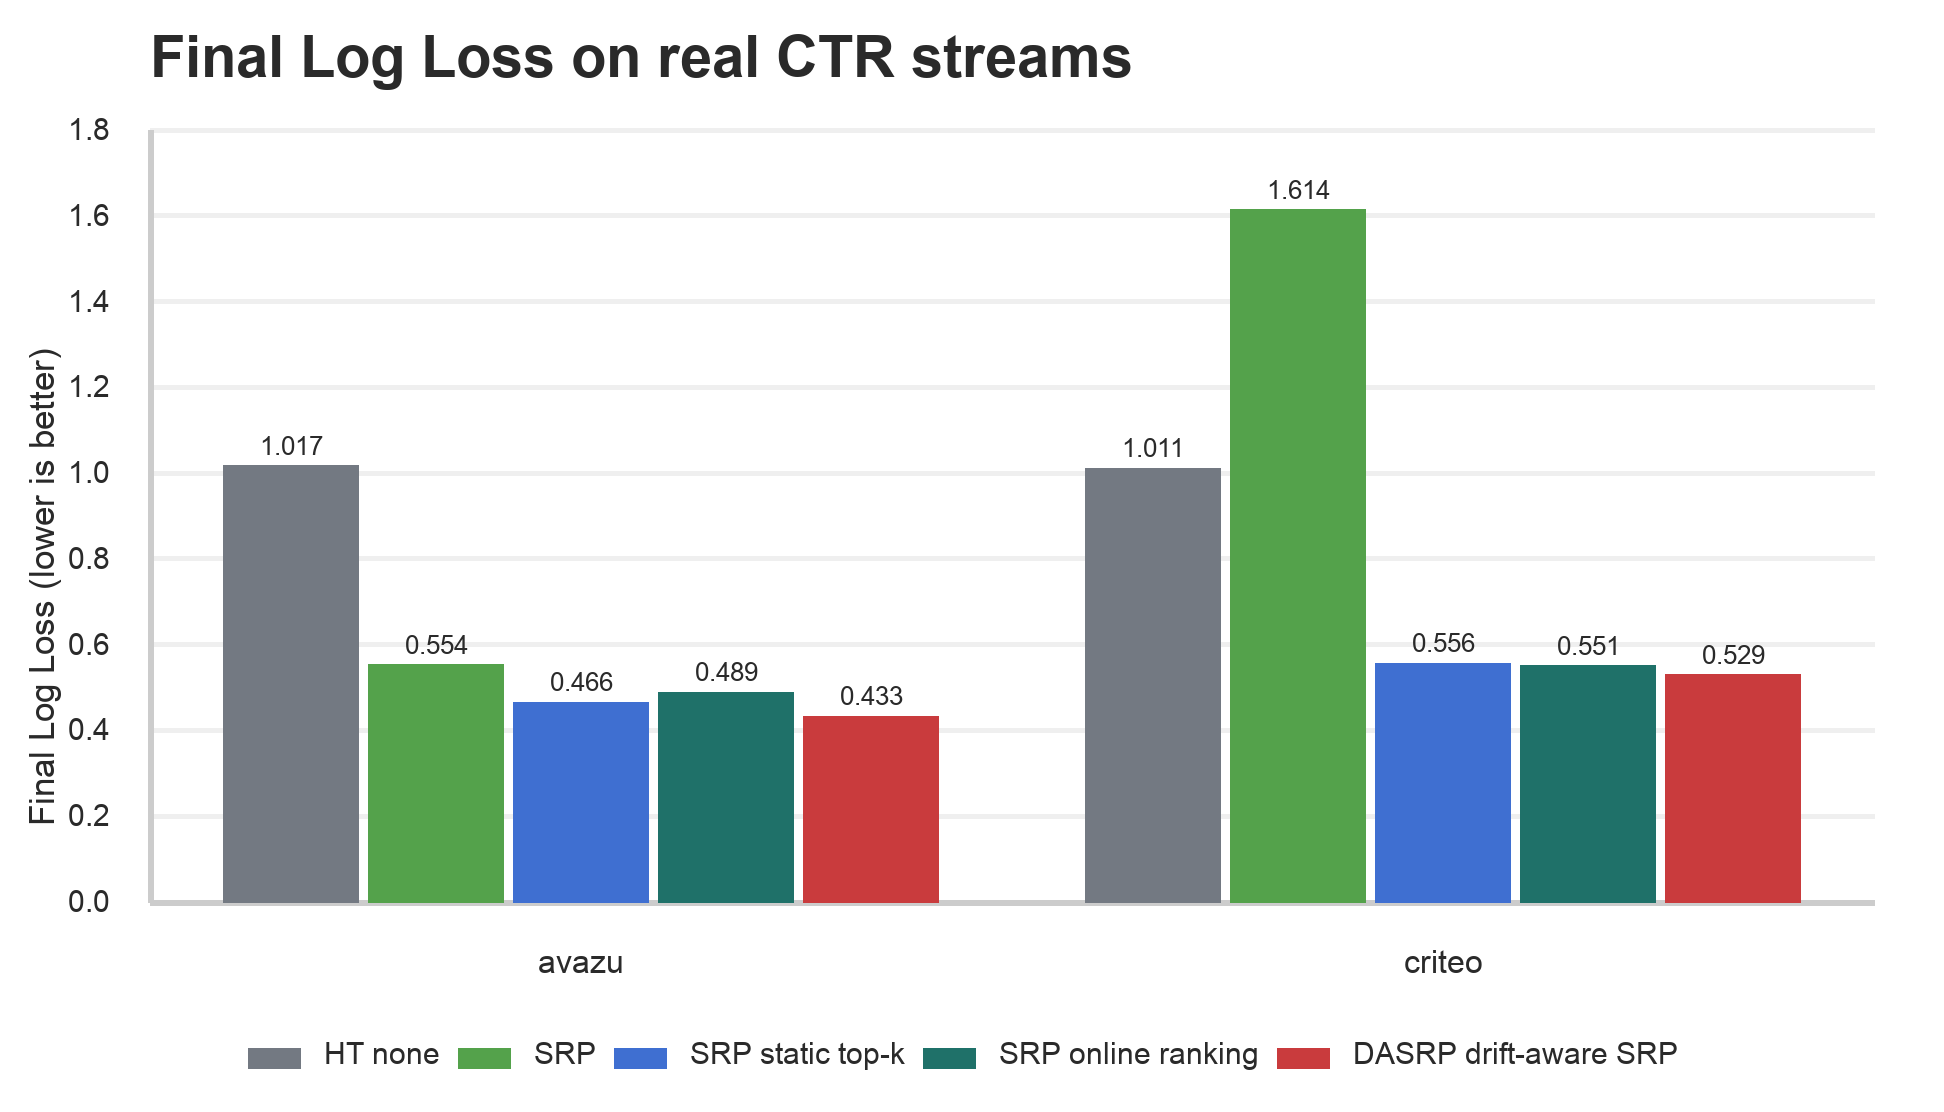
\includegraphics[width=0.95\linewidth]{figures/evaluation/eval_real_final_logloss_with_srp.png}
\caption{Final Log Loss comparison on Avazu and Criteo, including the SRP baseline.}
\label{fig:eval_real_final_logloss}
\end{figure}

The time-series view in Figure~\ref{fig:eval_real_windowed_logloss} shows that
the improvement is not only a final-point artifact. DASRP remains among the
lowest-loss methods throughout the real CTR streams. The Avazu result is
particularly stable. On Criteo, static SRP is competitive early but degrades
later, while DASRP avoids the strongest late loss increase.

\begin{figure}[H]
\centering
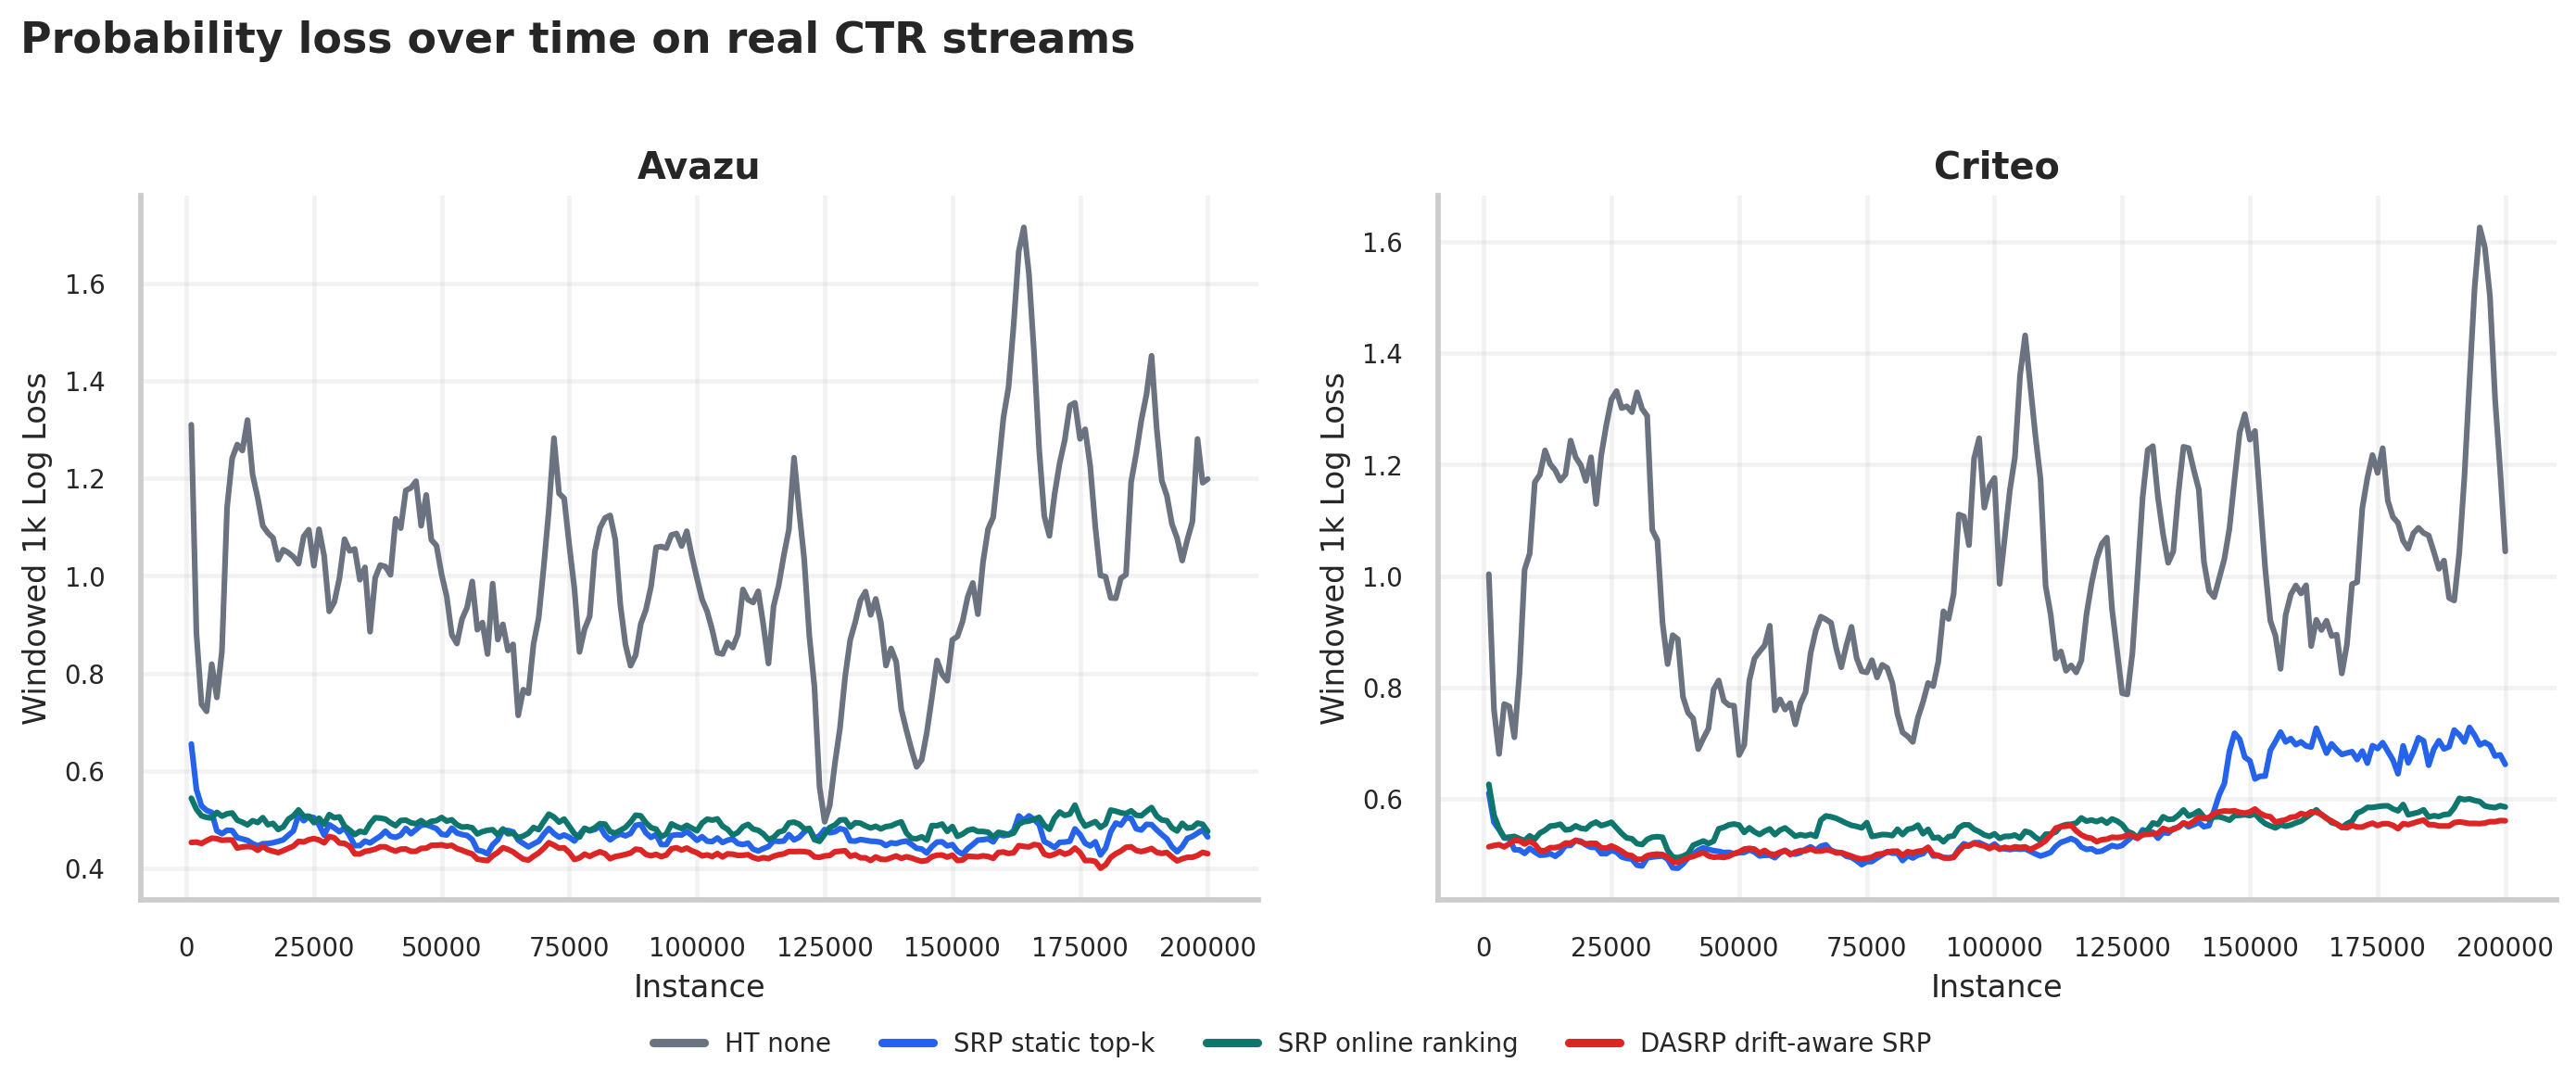
\includegraphics[width=\linewidth]{figures/evaluation/eval_real_windowed_logloss.png}
\caption{\new{Left: Avazu dataset. Right: Criteo dataset.} Windowed 1,000-instance Log Loss over time on real CTR streams:} 
\label{fig:eval_real_windowed_logloss}
\end{figure}


\subsection{Runtime analysis}
Runtime is a key constraint in streaming systems. A model that provides good
Log Loss but cannot process the stream fast enough is not practical. DASRP was
much faster than the strongest SRP baselines on real CTR streams \new{because it
uses a compact custom ensemble and, on drift, repairs only the subspaces of the
affected learners, instead of running the heavier vanilla SRP baseline
configuration with its per-learner background trees and detectors.}

\begin{figure}[H]
\centering
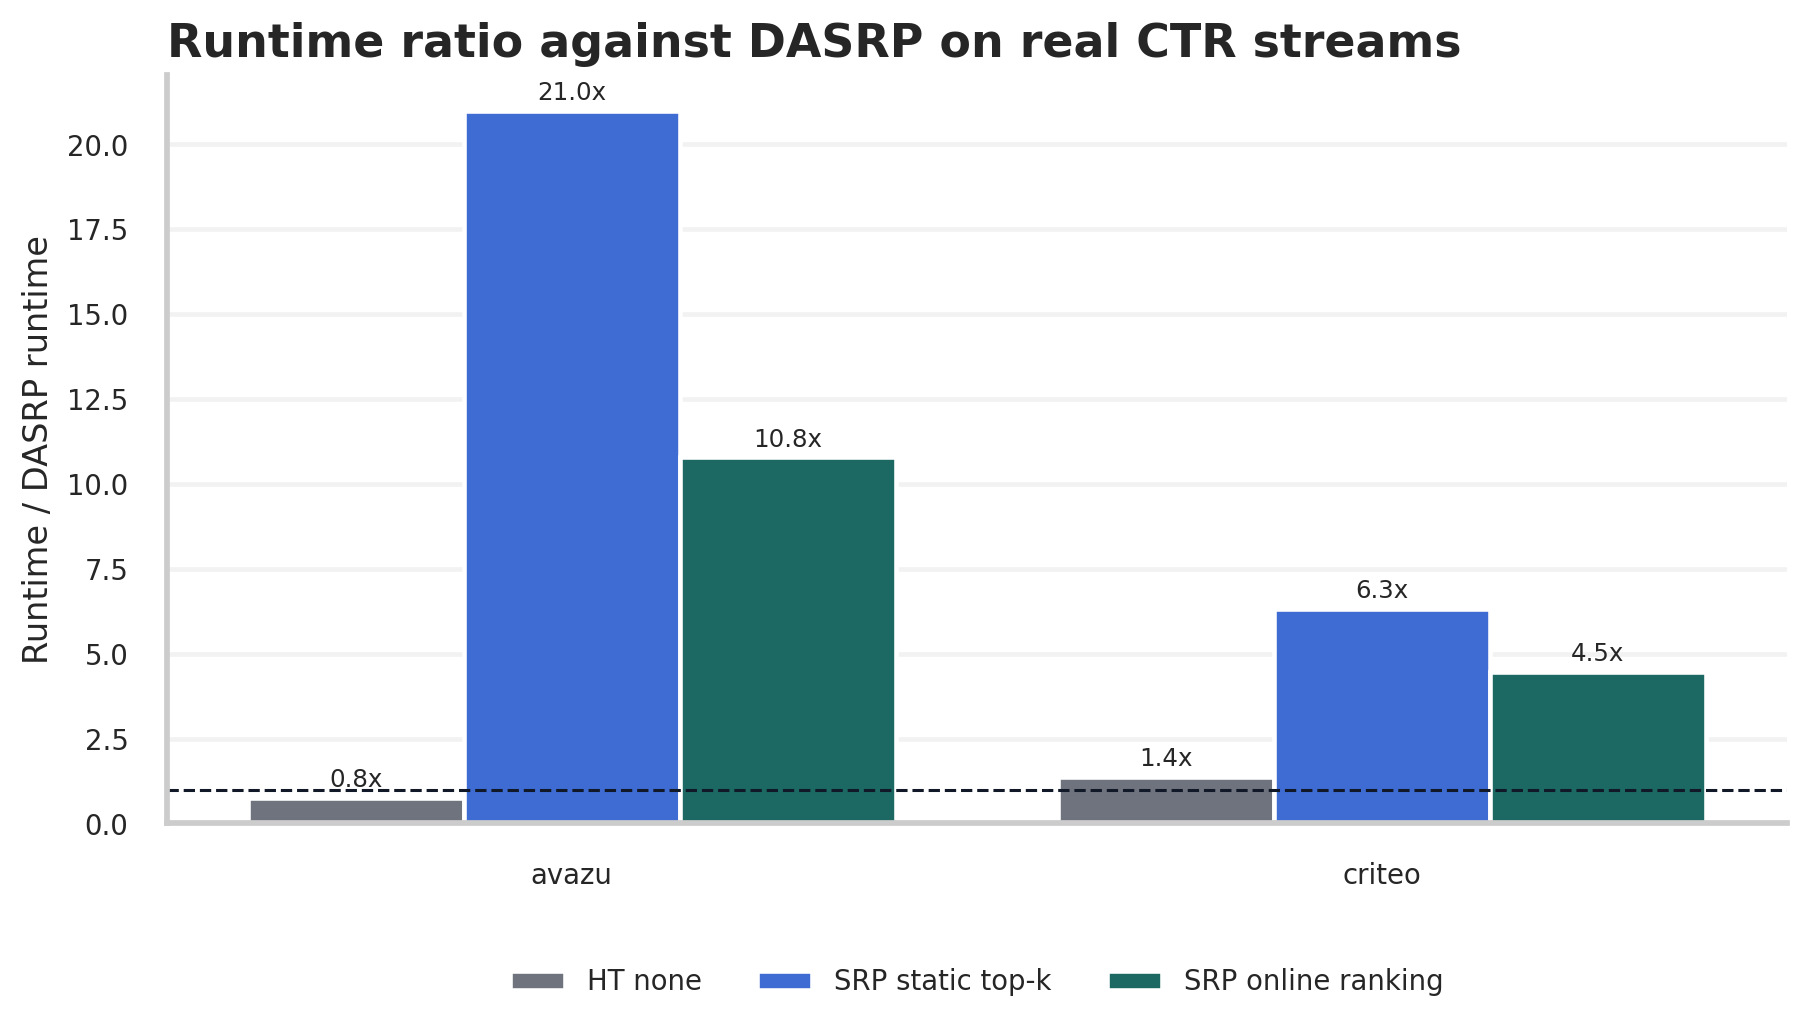
\includegraphics[width=0.85\linewidth]{figures/evaluation/eval_real_speedup_vs_dasrp.png}
\caption{\new{Avazu and Criteo datasets:} Runtime ratio of selected real-stream baselines against DASRP. Values
above 1 mean the baseline was slower than DASRP.}
\label{fig:eval_real_speedup}
\end{figure}

On Avazu, \new{SRP with static top-K took approximately 12.7 times the DASRP
runtime, and SRP with online ranking took approximately 6.0 times the DASRP
runtime}. HT
was faster than DASRP, but it was much worse in final Log Loss. This indicates
that DASRP is not the fastest method overall, but it provides an attractive
quality/runtime trade-off among the competitive ensemble methods.

\begin{figure}[H]
\centering
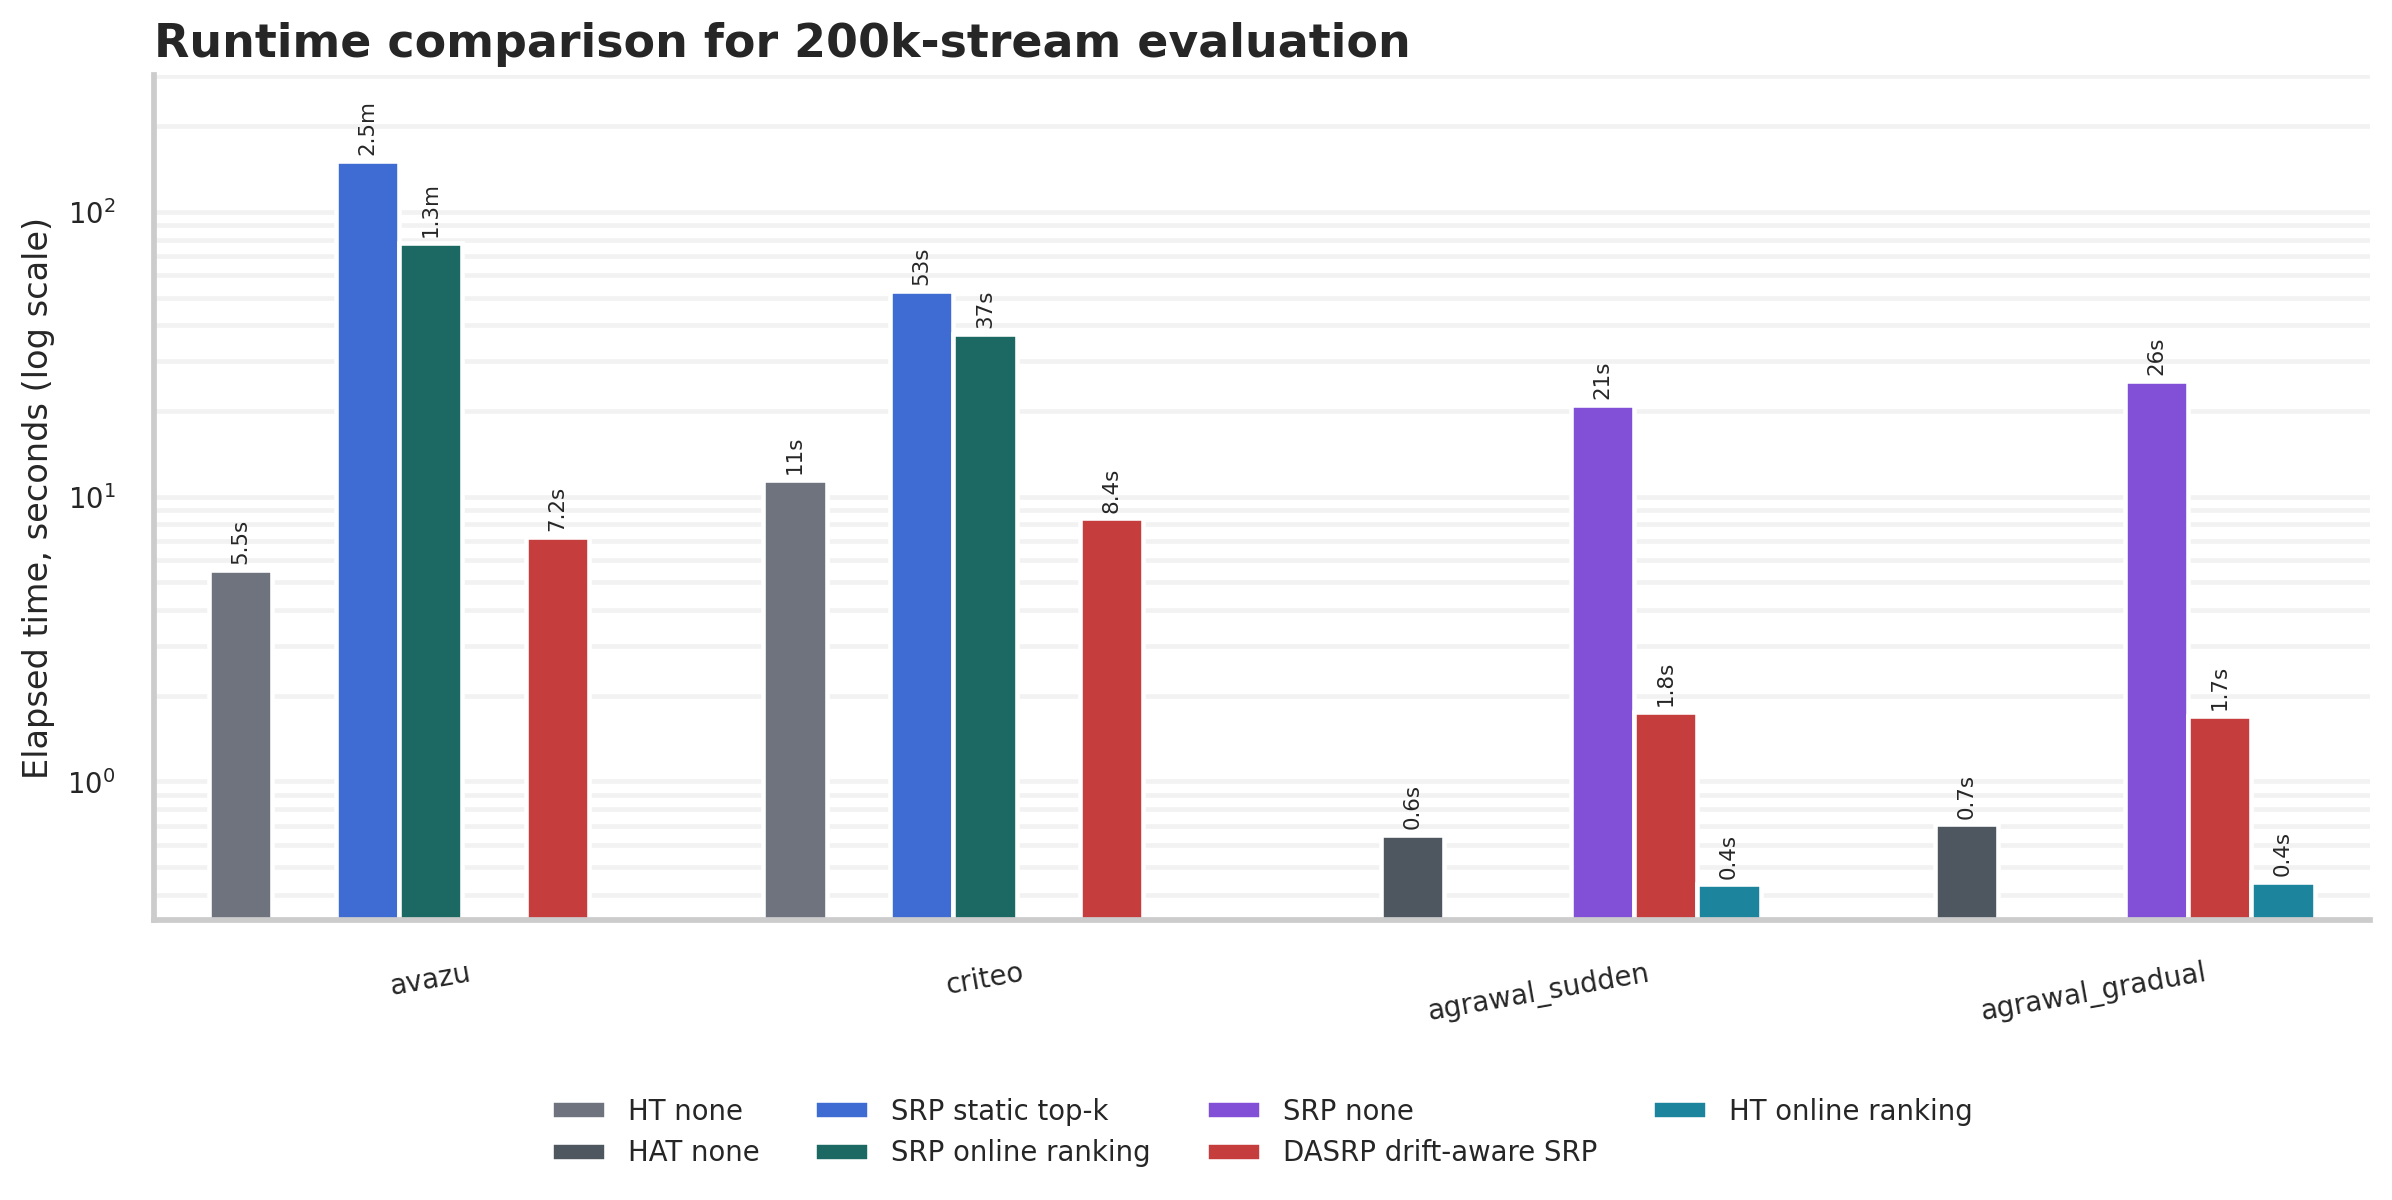
\includegraphics[width=\linewidth]{figures/evaluation/eval_runtime_comparison.png}
\caption{\new{Avazu and Criteo datasets.} Absolute runtime comparison for 200,000-instance runs. The vertical axis is logarithmic.}
\label{fig:eval_runtime_comparison}
\end{figure}

\subsection{\new{Synthetic-stream results}}
\label{subsec:synth_res}

\begin{table}[H]
\centering
\caption{\new{Final metrics on controlled synthetic streams. For each stream,
the strongest baseline by final Log Loss is compared with DASRP.}}
\label{tab:agrawal_final_metrics}
\begin{tabular}{llccc}
\toprule
Dataset & Method & Accuracy & Log Loss & AUC \\
\midrule
\new{Sudden Agrawal} & \new{HAT + no selector} & \new{\textbf{0.9978}} & \new{\textbf{0.0118}} & \new{\textbf{1.0000}} \\
\new{Sudden Agrawal} & \new{DASRP + drift-aware SRP} & \new{0.8311} & \new{0.3809} & \new{0.8860} \\
\midrule
\new{Gradual Agrawal} & \new{HAT + no selector} & \new{\textbf{0.9688}} & \new{\textbf{0.1123}} & \new{1.0000} \\
\new{Gradual Agrawal} & \new{DASRP + drift-aware SRP} & \new{0.9572} & \new{0.3191} & \new{\textbf{1.0000}} \\
\midrule
\new{Noisy Agrawal} & \new{HAT + no selector} & \new{\textbf{0.9203}} & \new{\textbf{0.2651}} & \new{\textbf{0.9871}} \\
\new{Noisy Agrawal} & \new{DASRP + drift-aware SRP} & \new{0.7757} & \new{0.4869} & \new{0.8667} \\
\midrule
\new{LED irrelevant} & \new{SRP + static top-K} & \new{0.1887} & \new{\textbf{3.0126}} & \new{0.7647} \\
\new{LED irrelevant} & \new{DASRP + drift-aware SRP} & \new{\textbf{0.1954}} & \new{3.2834} & \new{\textbf{0.9360}} \\
\midrule
\new{RBF highdim} & \new{SRP + no selector} & \new{\textbf{0.9988}} & \new{\textbf{0.0084}} & \new{\textbf{1.0000}} \\
\new{RBF highdim} & \new{DASRP + drift-aware SRP} & \new{0.9250} & \new{0.2270} & \new{0.9672} \\
\bottomrule
\end{tabular}
\end{table}

\new{The expanded synthetic evaluation satisfies the mandatory condition of
testing reference and novel methods on several controlled streams. The results
also reveal an important limitation: DASRP is not universally superior on
simple synthetic generators. On Agrawal and RBF, the best reference baselines
learn the generated concepts very quickly. DASRP is competitive on gradual
Agrawal but underperforms on the noisier and high-dimensional RBF settings
because frequent drift alarms cause too many feature/subspace repairs. On LED,
where the relevant and irrelevant attributes are explicitly swapped, DASRP
substantially reduces Log Loss compared with most tree baselines and is close
to the best SRP top-K configuration.}

\begin{figure}[H]
\centering
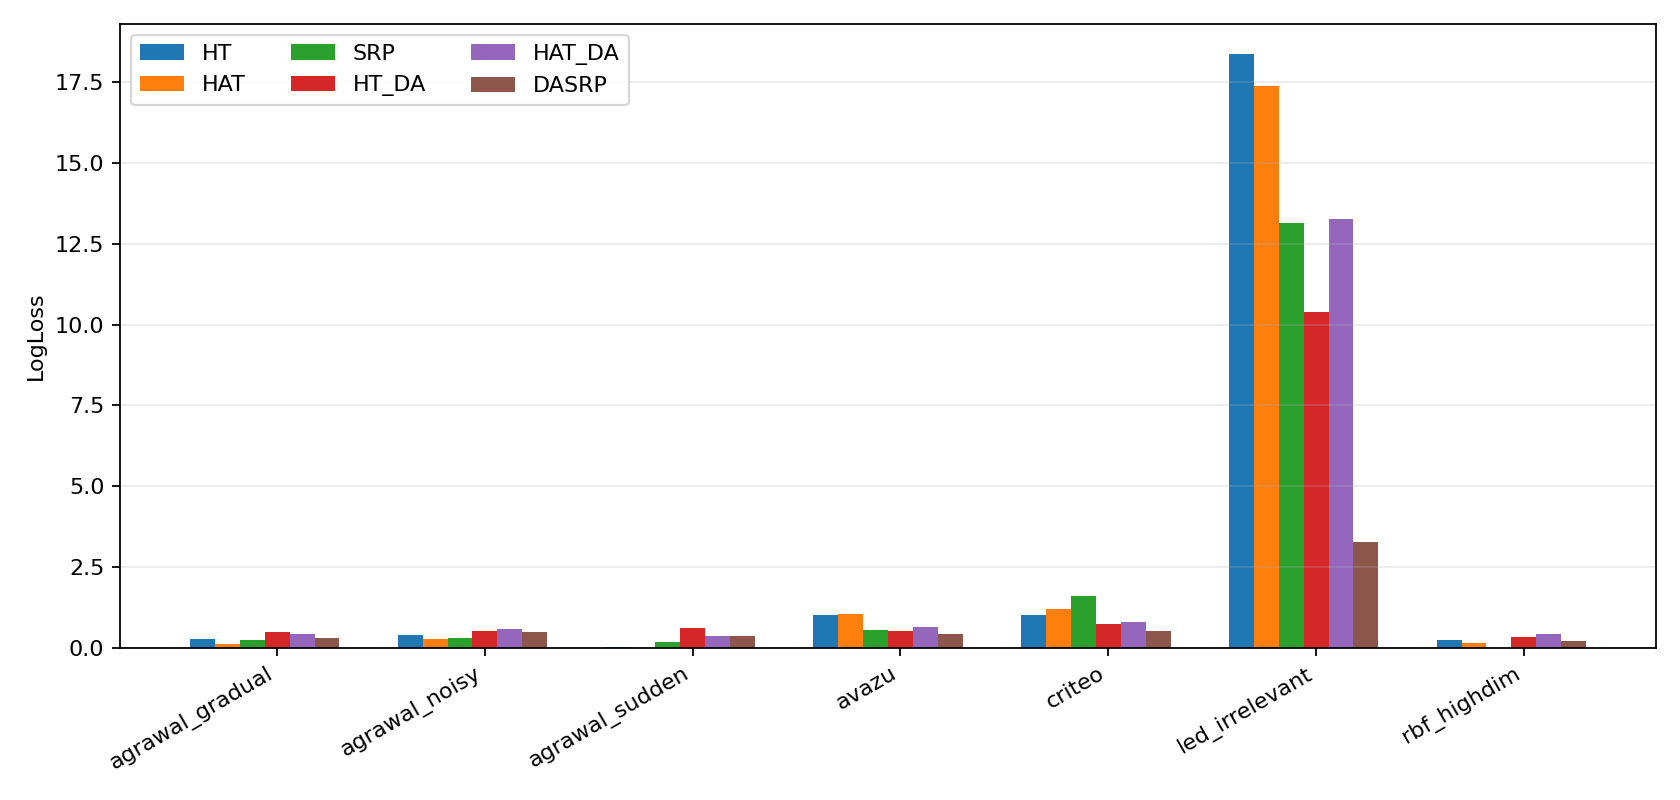
\includegraphics[width=\linewidth]{plots/model_comparison_logloss.png}
\caption{\new{All seven evaluated datasets: final Log Loss for HT, HAT, vanilla
SRP, HT with drift-aware selection, HAT with drift-aware selection, and DASRP.
This plot explicitly includes vanilla SRP in the synthetic comparison.}}
\label{fig:model_comparison_logloss_all}
\end{figure}

\begin{figure}[H]
\centering
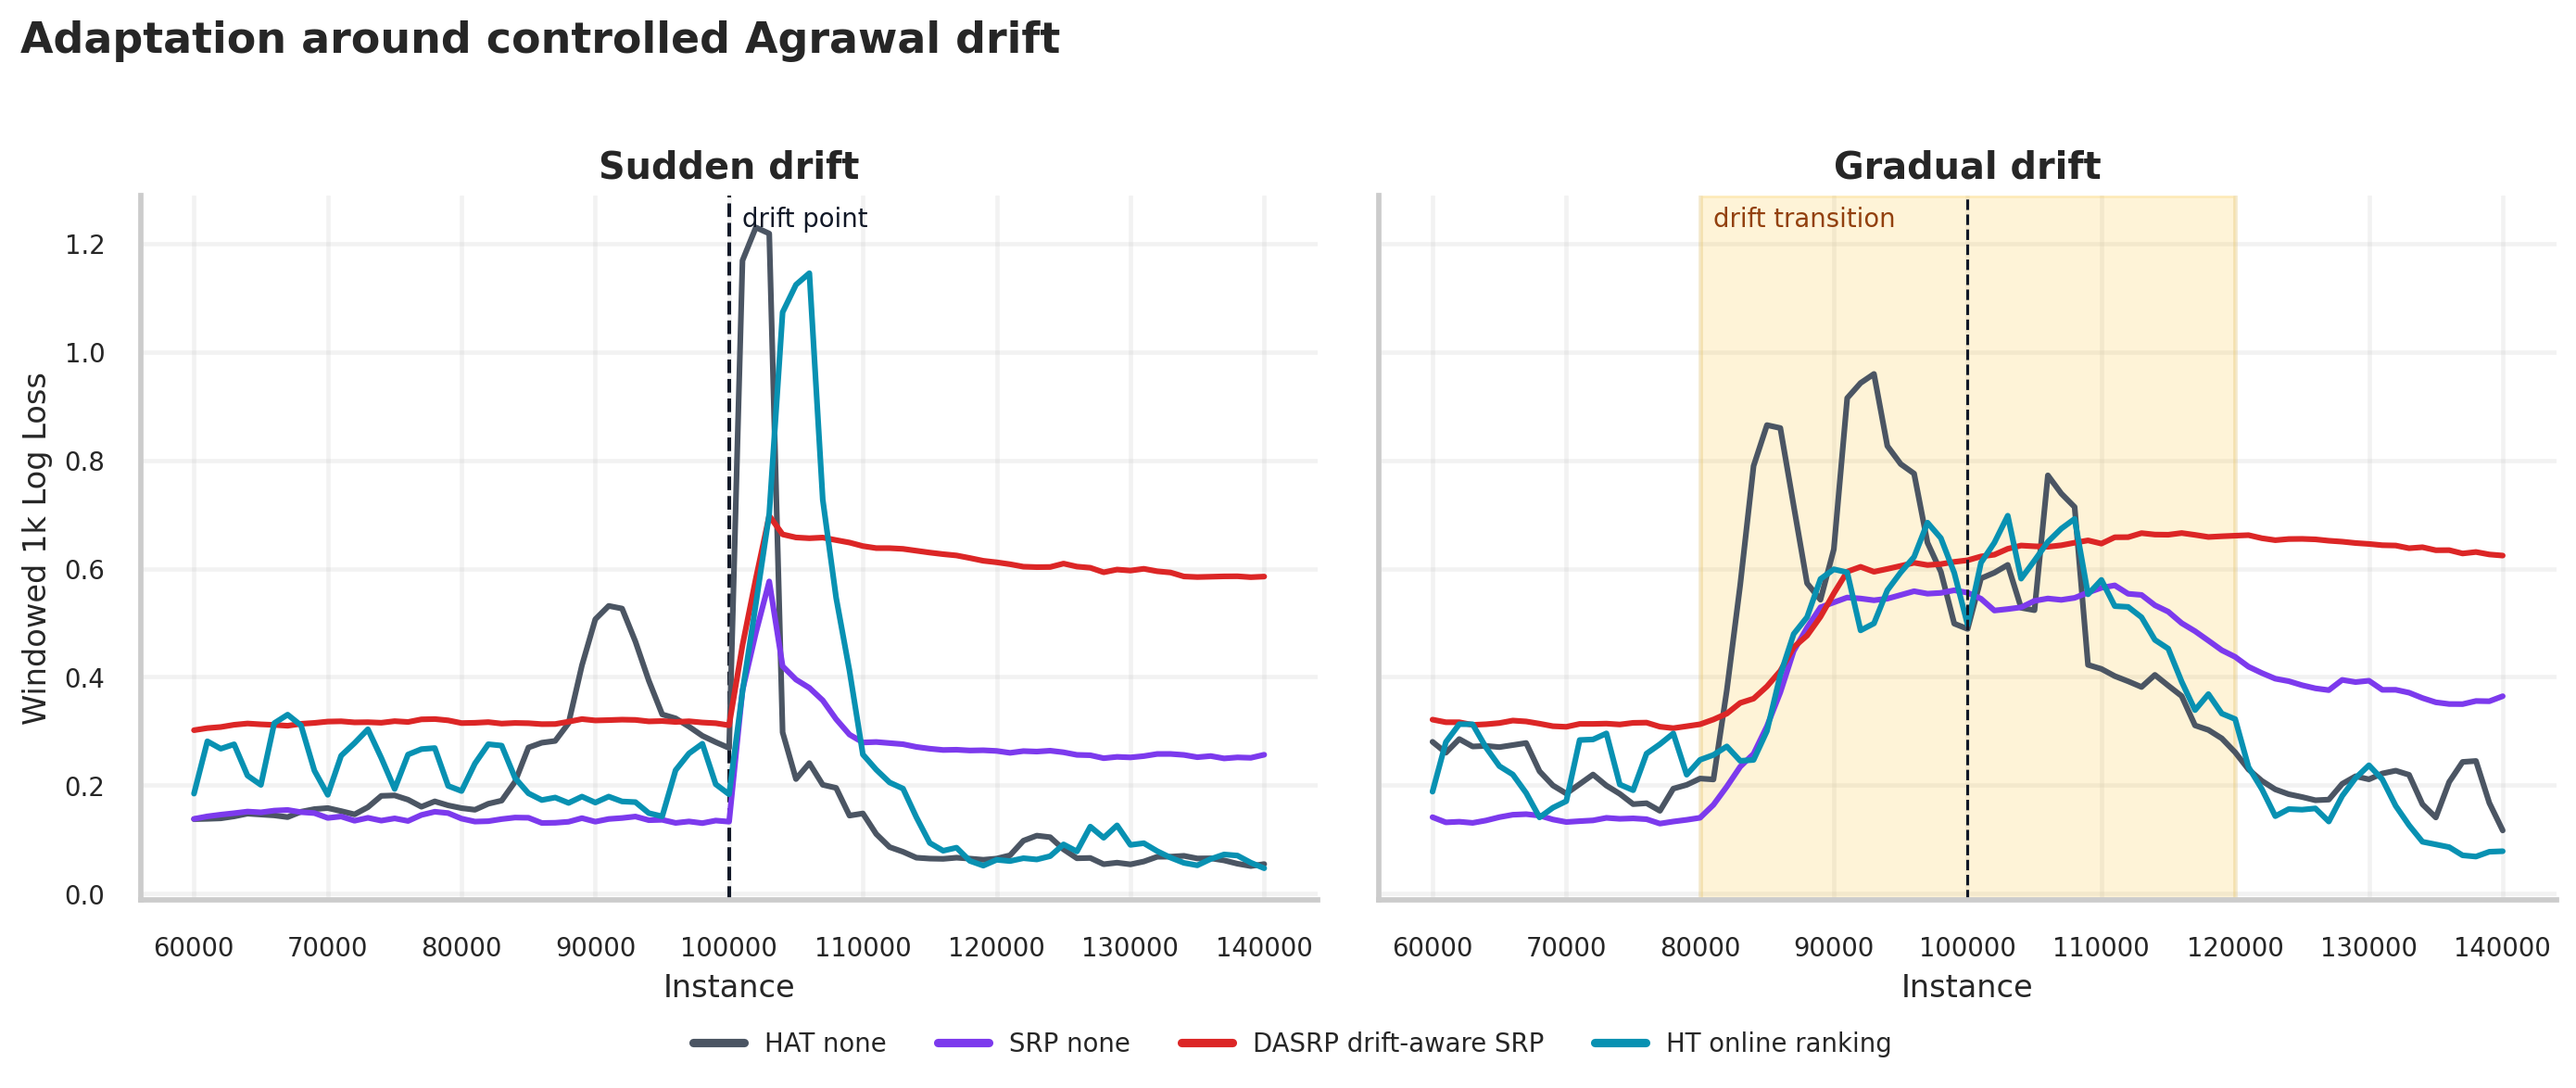
\includegraphics[width=\linewidth]{figures/evaluation/eval_synthetic_adaptation.png}
\caption{\new{Agrawal sudden and gradual datasets:} Windowed Log Loss around controlled Agrawal drift.}
\label{fig:eval_synthetic_adaptation}
\end{figure}

The number of ADWIN alarms also shows that drift-aware mechanisms require
careful tuning. In simple synthetic streams, frequent alarms may lead to
unnecessary feature and model changes.

\begin{figure}[H]
\centering
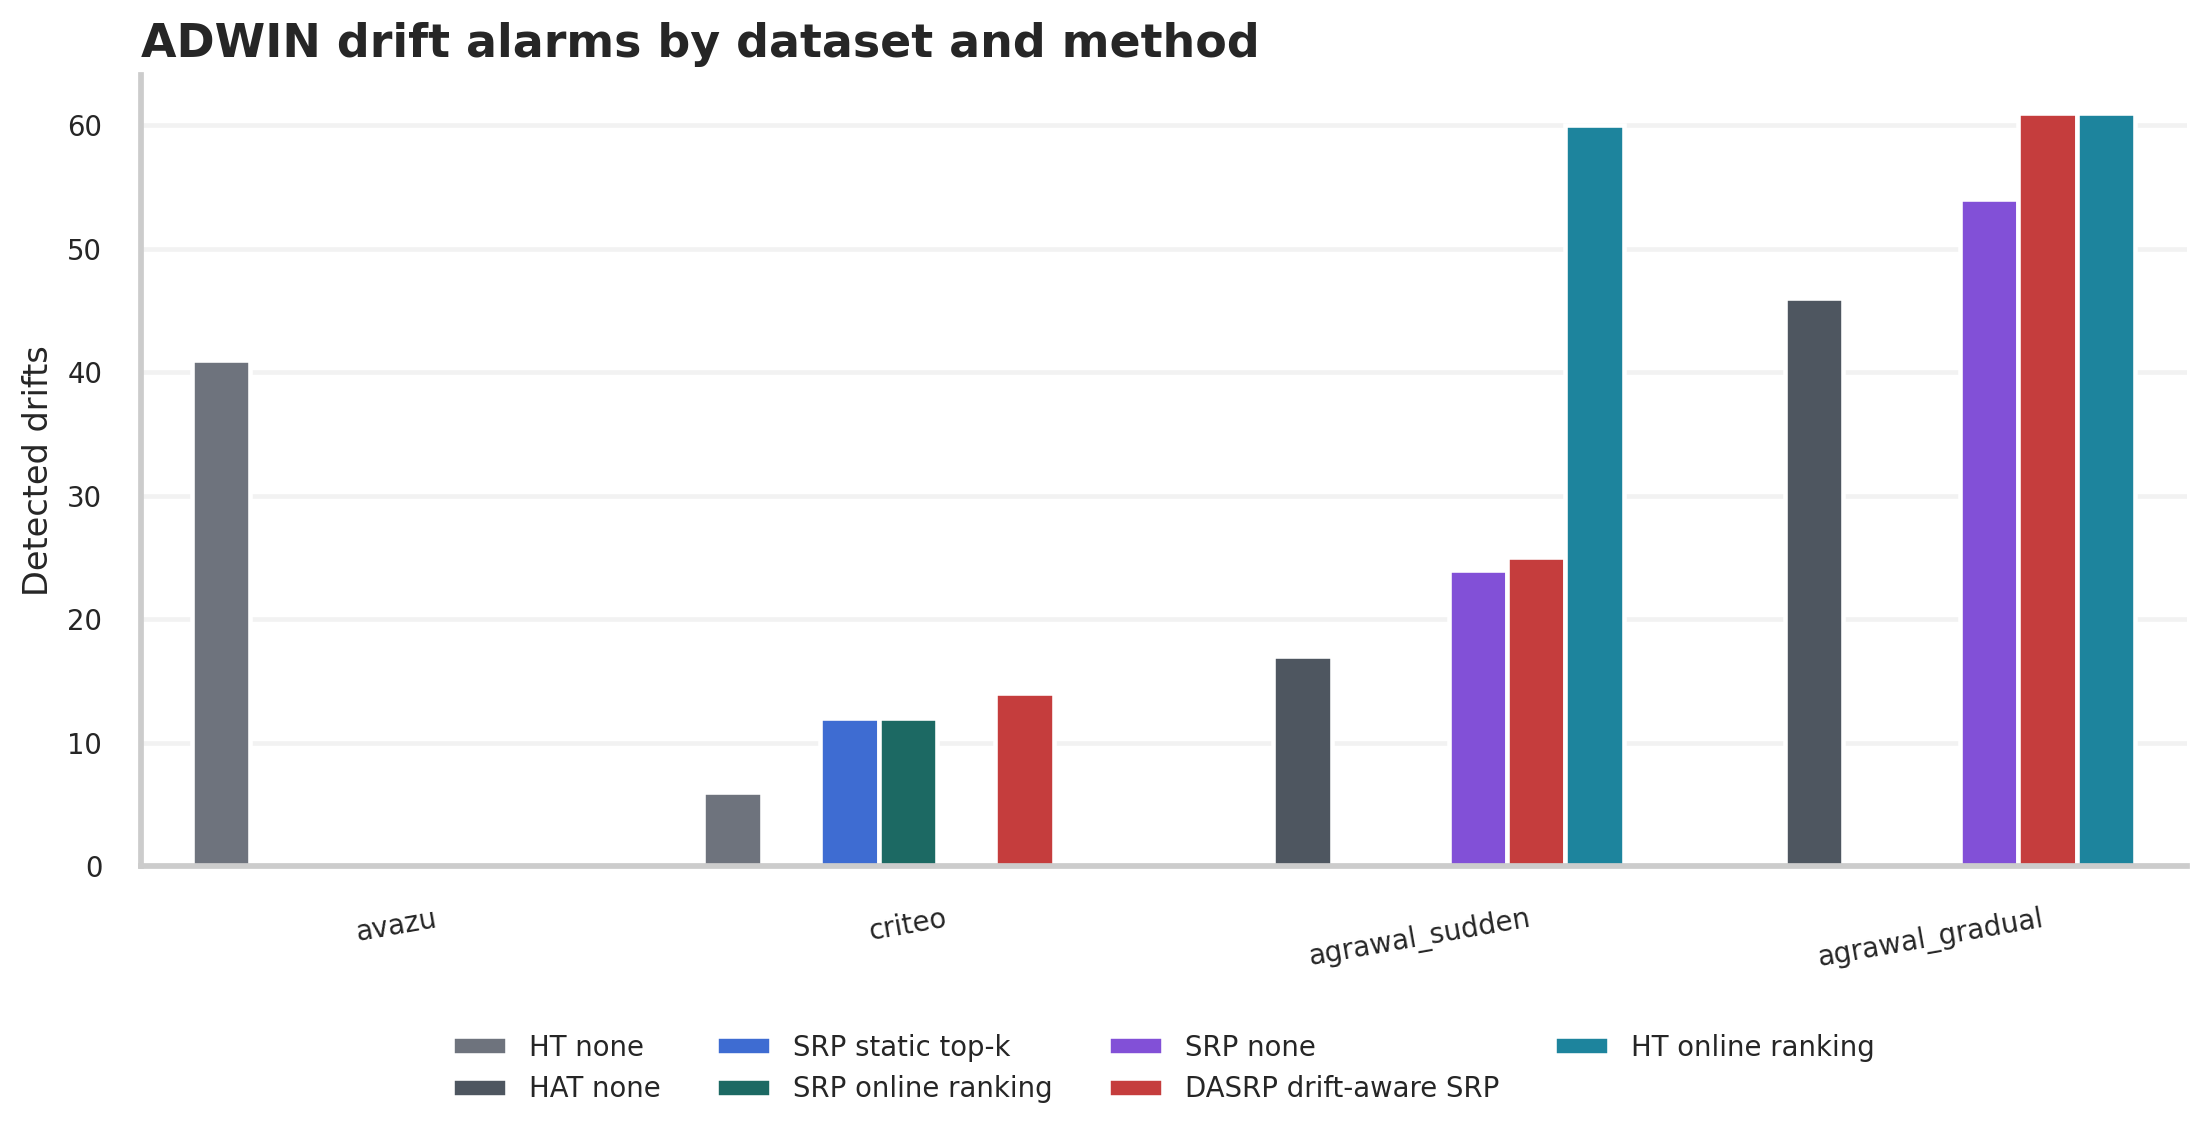
\includegraphics[width=0.95\linewidth]{figures/evaluation/eval_drift_counts.png}
\caption{\new{All evaluated datasets:} ADWIN drift alarms by dataset and selected method.}
\label{fig:eval_drift_counts}
\end{figure}

\section{Conclusion}
\label{sec:conc}

The final experiments confirm that online feature adaptation can improve CTR
prediction in high-dimensional, non-stationary streams. On Avazu and Criteo,
DASRP achieved the best final Log Loss among the evaluated methods and was
substantially faster than the strongest SRP baselines. This is the most
important outcome of the project because CTR systems rely on calibrated
probabilities rather than only hard class labels.

\new{The expanded synthetic experiments provide an important limitation. On
Agrawal and RBF streams, standard adaptive trees or vanilla SRP can recover very
well because the generated concepts are comparatively clean and quickly
learnable. DASRP is therefore not universally superior. Its strongest use case
is a stream where feature relevance itself is unstable and where selective
subspace repair avoids the high cost of rebuilding a full ensemble. The LED
irrelevant-attribute experiment supports this interpretation, while the noisy
and high-dimensional synthetic runs show that ADWIN and IG thresholds require
careful per-stream tuning.}

\new{Future work should include full million-instance experiments, a formal
recovery-time metric around drift events, feature-level drift detectors in
addition to the current error-rate ADWIN, and a more systematic search over
ADWIN sensitivity, Information Gain thresholds, subspace sizes, reset ratio, and
weight recovery rate.}

\section{Team contributions}
\label{app:contrib-clean}

\begin{table}[H]
\centering
\caption{Division of work across team members, including detailed contributions and time assessment.}
\label{tab:contrib-clean}
\resizebox{\linewidth}{!}{%
\begin{tabular}{|l|>{\raggedright\arraybackslash}p{0.65\linewidth}|c|}
\hline
\textbf{Name} & \textbf{Contributions} & \textbf{Workload} \\
\hline
Hubert Jaczy\'nski & \textbf{Analytics and final evaluation:} concept drift detection in raw data with ADWIN; final evaluation and comparative analysis of the proposed algorithm against baselines. \textbf{Report:} final evaluation and conclusion sections. \textbf{Presentation creation.} \new{\textbf{Revision:} added Hoeffding Tree results to the real CTR table, added the SRP + online ranking row for Avazu, produced the model-comparison plot including vanilla SRP, extended the synthetic-stream results and drift-count analysis, and clarified the error-rate basis of the ADWIN alarms.} & $\sim$45h\\
\hline
Aleksandra K{\l}os & \textbf{Data engineering and baseline evaluation:} preprocessing Avazu and Criteo streams, exploratory data analysis, feature hashing, missing-value imputation, baseline evaluation in MOA, and scripts for Log Loss and adaptation-gap analysis. \textbf{Report:} introduction, data preparation, and evaluation methodology sections. \textbf{Presentation creation.} \new{\textbf{Revision:} corrected the Criteo rolling-statistics computation so it is performed before zero-imputation and regenerated the ARFF file, added dataset names to all figure captions, fixed and described the \texttt{site\_x\_hour} feature, regenerated the HT adaptation-gap experiment at the consistent 200{,}000-instance scale, and added the comment on additional drift types in Subsection~\ref{subsec:drift}.} & $\sim$45h \\
\hline
Jakub Oganowski & \textbf{Algorithm implementation:} Java implementation of the SRP/OFS integration, drift-aware feature selection, subspace adaptation, and ensemble weighting. \textbf{Report:} architecture of the proposed solution section. \textbf{Presentation creation.} \new{\textbf{Revision:} added the \texttt{algorithm2e} pseudocode for the main pipeline and the drift-aware selector, implemented the three new synthetic stream providers (noisy Agrawal, LED, high-dimensional RBF), clarified the single error-rate ADWIN input and the model-reset behaviour, and documented the safeguard against low Information Gain features by replacing high Information Gain ones.} & $\sim$45h \\
\hline
\end{tabular}%
}
\end{table}


\section{Updates compared to the preliminary report}
\label{sec:response}

{\color{blue}
All newly added or revised content is highlighted in blue throughout the report.
Table~\ref{tab:changes} maps each reviewer remark to the section(s) modified.

\footnotesize
\begin{longtable}{|>{\raggedright\arraybackslash}p{0.31\textwidth}
                |>{\raggedright\arraybackslash}p{0.41\textwidth}
                |>{\raggedright\arraybackslash}p{0.18\textwidth}|}
\caption{Changes addressed in response to the reviewer comments.}
\label{tab:changes}\\
\hline
\textbf{Reviewer remark} & \textbf{Change applied} & \textbf{Changed section(s)} \\
\hline
\textit{Add pseudocode, e.g. with algorithm2e, for the main pipeline and
drift-aware feature selection.}
&
Added two \texttt{algorithm2e} blocks: the prequential evaluation/adaptation
pipeline and the ADWIN-triggered drift-aware feature-selection procedure.
\new{In the second revision, Algorithm~\ref{alg:main_pipeline} now explicitly
shows that a monolithic model is reinitialised on the new filtered header when
the selector changes the subset (DASRP instead repairs only the affected
subspaces); Algorithm~\ref{alg:drift_aware_selector} was corrected so that
$S_{base}$ initialises $S_{new}$ and that $S_{old}$/$S_{new}$ are defined input
and output sets used to form the removed/added sets; and the LED subspace size
of 7 is no longer justified by the ground-truth relevant-attribute count but
flagged as an oracle-informed diagnostic setting.}
&
Subsection~\ref{subsec:stream_pip}, Algorithm~\ref{alg:main_pipeline}; Subsection~\ref{subsec:drift-aware},
Algorithm~\ref{alg:drift_aware_selector}\new{, Subsection~\ref{subsec:drift_aware_srp}}. \\
\hline
\textit{Clarify how feature selection influences existing models such as HT,
and whether past models are dropped or new splits are constrained.}
&
Clarified that HT, HAT, and vanilla SRP receive physically filtered instances.
When a dynamic selector changes the feature subset, the model is reinitialised
on a new filtered header; old splits are dropped, not retroactively constrained.
\new{For DASRP, every ensemble learner whose subspace is modified is likewise
reinitialised; the reset ratio only controls which of those learners also have
their voting weight temporarily reduced.}
&
Subsection~\ref{subsec:baseline}, Subsection~\ref{subsec:drift-aware}\new{, and
Subsection~\ref{subsec:drift_aware_srp}}. \\
\hline
\textit{Clarify the input of ADWIN. Is there one ADWIN instance per feature?}
&
Clarified that the Java evaluation uses one ADWIN detector per evaluated model
run. Its input is the online 0/1 prediction-error stream. There is not one
ADWIN instance per feature.
&
Subsection~\ref{subsec:drift-aware} and Algorithm~\ref{alg:main_pipeline}. \\
\hline
\textit{Add dataset names to plot captions; fix \texttt{site\_x\_hour}; explain
how IG is computed and based on what data.}
&
Added dataset names to captions, fixed the \texttt{site\_x\_hour} formatting,
defined it as a site/hour interaction, and described IG estimation on warm-up,
sliding, pre-drift, and post-drift buffers. \new{In the second revision we
additionally defined \texttt{site\_id}, \texttt{app\_id} and \texttt{device\_type}
as raw Avazu columns, listed all three \texttt{*\_x\_hour} interaction features
explicitly, and clarified that the four sliding-window CTR/frequency statistics
are numeric attributes added to the data (part of the 109 Avazu features).}
&
\new{Subsection~\ref{subsec:feat},} Subsection~\ref{subsec:synth}, Subsection~\ref{subsec:drift}, Subsection~\ref{subsec:baseline}, figure captions. \\
\hline
\textit{Reconsider Criteo rolling statistics because imputed values may disturb
the calculations.}
&
Clarified and revised the preprocessing description: rolling statistics for
\texttt{I1}--\texttt{I5} are computed before zero-imputation, with missing
values skipped by the window estimator. Remaining missing original values are
then zero-filled.
&
Subsection~\ref{subsec:synth}. \\
\hline
\textit{Add at least three more synthetic streams, including one larger
dimensionality stream.}
&
Added \texttt{agrawal\_noisy}, \texttt{led\_irrelevant}, and
\texttt{rbf\_highdim}. The RBF stream has 100 attributes. The final evaluation
now contains 63 baseline and 21 drift-aware runs over seven datasets.
&
Subsection~\ref{subsec:summ}, Table~\ref{tab:datasets_summary}, Subsection~\ref{subsec:matrix}, Subsection~\ref{subsec:synth_res}. \\
\hline
\textit{Comment whether drift detected in Subsection~\ref{subsec:baseline} is the only drift present;
add drift detection experiments based on other features and error rates.}
&
Added an explicit comment that CTR drift is not the only possible drift. The
main Java experiments additionally log ADWIN alarms from model error-rate
streams, and the final evaluation reports drift counts by dataset and method.
&
Subsection~\ref{subsec:drift}, Subsection~\ref{subsec:drift-aware}, Fig.~\ref{fig:eval_drift_counts}. \\
\hline
\textit{Use Hoeffding Tree as another baseline.}
&
Added HT to the baseline model set and explicitly included HT rows in the real
CTR result table. HT is also included in the committed 63-run baseline
summary.
&
Subsection~\ref{subsec:baseline}, Table~\ref{tab:real_final_metrics}, Subsection~\ref{subsec:matrix}. \\
\hline
\textit{SRP + online ranking results are missing for Avazu.}
&
Added the Avazu SRP + online ranking row to the real CTR result table and kept
the corresponding row in the committed results CSV.
&
Table~\ref{tab:real_final_metrics}; \path{results_summary.csv}. \\
\hline
\textit{Could a feature of low yet growing IG replace a high-IG feature that is
not improving? Consider modifying the mechanism.}
&
Clarified the implemented safeguard: the selected set is anchored in the
post-drift top-$K$ ranking and is shrunk by $IG_{after}$ if it grows beyond
$K$. Thus a low-IG feature cannot replace a still-high-IG feature solely
because its IG increased.
&
Subsection~\ref{subsec:drift-aware}. \\
\hline
\textit{Fig. 11 should include vanilla SRP.}
&
Added a final Log Loss comparison plot over all seven datasets that explicitly
contains vanilla SRP together with HT, HAT, HT-DA, HAT-DA, and DASRP.
&
Fig.~\ref{fig:model_comparison_logloss_all}, Subsection~\ref{subsec:synth_res}. \\
\hline
\textit{DASRP may drop relevant features. Analyse which features are left and
possibly revise DASRP.}
&
Clarified that DASRP repairs only learners whose subspaces overlap sufficiently
with weakened features. Unaffected learners preserve their old subspaces. The
final discussion also identifies over-adaptation under frequent alarms as a
limitation requiring per-stream threshold calibration.
&
Subsection~\ref{subsec:drift_aware_srp}, Subsection~\ref{subsec:synth_res}, Conclusion. \\
\hline
\end{longtable}
}

\appendix
\section{Github repository link}

\new{Most of the data, code, results, and synthetic data stream configurations
developed for this project are available in the following repository:}

\begin{center}
\url{https://github.com/Klossek02/MLDataStreams}
\end{center}


\printbibliography

\listoffigures

\listoftables


\end{document}
